%\documentclass[sigconf]{acmart}

\documentclass[conference]{IEEEtran}
\usepackage[hyperfootnotes=false]{hyperref}
% to be able to draw some self-contained figs
%\usepackage{tikz}
%\usepackage{amsmath}
% inlined bib file
\usepackage[listings,skins,breakable]{tcolorbox}
\usepackage{amsmath,amssymb}
\usepackage{booktabs}
\usepackage{algorithm}
\usepackage[noend]{algpseudocode}
\usepackage{jimola}
\usepackage{xcolor}
\usepackage{comment}
\usepackage{subcaption}
\usepackage{multirow}

\newcommand{\ji}[1]{\textcolor{red}{ JI: #1}}
\newcommand{\arc}[1]{\textcolor{blue}{ ARC: #1}}
\newcommand{\kc}[1]{\textcolor{magenta}{KC: #1}}
\def\threshresp{{m + \sqrt{2\rho n \ln \frac{4n}{\delta}}}}
\def\threshresphybrid{{m + \sqrt{2\rho n \ln \frac{8n}{\delta}}}}

\newcounter{savefootnote}
\newcounter{symfootnote}
\newcommand{\symfootnote}[1]{%
   \setcounter{savefootnote}{\value{footnote}}%
   \setcounter{footnote}{\value{symfootnote}}%
   \ifnum\value{footnote}>8\setcounter{footnote}{0}\fi%
   \let\oldthefootnote=\thefootnote%
   \renewcommand{\thefootnote}{\fnsymbol{footnote}}%
   \footnote{#1}%
   \let\thefootnote=\oldthefootnote%
   \setcounter{symfootnote}{\value{footnote}}%
   \setcounter{footnote}{\value{savefootnote}}%
}
%-------------------------------------------------------------------------------
\begin{document}
%-------------------------------------------------------------------------------

%don't want date printed
%\date{}

% make title bold and 14 pt font (Latex default is non-bold, 16 pt)
\title{\Large \bf Robustness of Locally Differentially Private Graph Analysis Against Poisoning}

%for single author (just remove % characters)
%\author{{\rm Jacob Imola$^*$}\\UC San Diego \and {\rm Amrita Roy Chowdhury$^*$}\\UC San Diego\and  {\rm Kamalika Chaudhuri}\\ UC San Diego}

\maketitle

%-------------------------------------------------------------------------------
\begin{abstract} \arc{Fix abstract}
 Locally differentially private (\ldp) graph analysis allows private analysis on a graph that is distributed across multiple users.  However, such computations are vulnerable to data poisoning attacks where an adversary can skew the results by submitting malformed data. In this paper, we formally study the impact of poisoning attacks for graph degree estimation protocols under \ldp. We make two key technical contributions. First, we observe \ldp~makes a protocol more vulnerable to poisoning -- the impact of poisoning is worse when the adversary can directly poison their (noisy) responses, rather than their input data. Second, we observe that graph data is naturally redundant -- every edge is shared between two users. Leveraging this data redundancy, we design robust degree estimation protocols under \ldp~that can significantly reduce the impact of data poisoning and compute degree estimates with high accuracy.  We evaluate our proposed robust degree estimation protocols under poisoning attacks on real-world datasets to demonstrate their efficacy in practice. 
\end{abstract}
\section{Introduction}\label{chap4-sec:intro}
 Federated analytics enable a data analyst to gather useful information from data distributed across multiple users \textit{without} centrally pooling the data. An important class of tasks in federated analytics  is computing statistics over graph data, which has wide-spread applications ranging from market value prediction~\cite{matsunaga2019exploring}, fake news detection~\cite{benamira2019semi} to drug development~\cite{gaudelet2021utilizing}.  Usually, the graph encodes sensitive user information, such as social network data, which raises privacy concerns.  For instance, a mobile phone company might be interested in calculating statistics over the graph of call history which reveals an user's social interactions. To this end, local differential privacy (\ldp) is currently the most popular model for achieving data privacy for federated analytics. %\ldp~has been deployed by major commercial organizations, such as Google~\cite{Rappor1,Rappor2}, Apple~\cite{Apple} and Microsoft~\cite{Microsoft}.\textcolor{white}{t\symfootnote{The first two authors have made equal contributions.}}

%Unfortunately, \ldp~brings forth a host of challenges. 

The distributed nature of \ldp, however, leaves the door open for poisoning attacks. For example, an adversary can inject fake users into the system or compromise the accounts of real users to run untrusted applications on user devices. Consequently, there is no guarantee that these users will comply with the \ldp~protocols. The adversary can send carefully crafted malformed data from these non-compliant users and skew statistical estimates, including those involving only honest users. 
%Additionally, such poisoning attacks can tamper with statistics that pertain to only the honest users. 
\begin{figure}
    \centering
    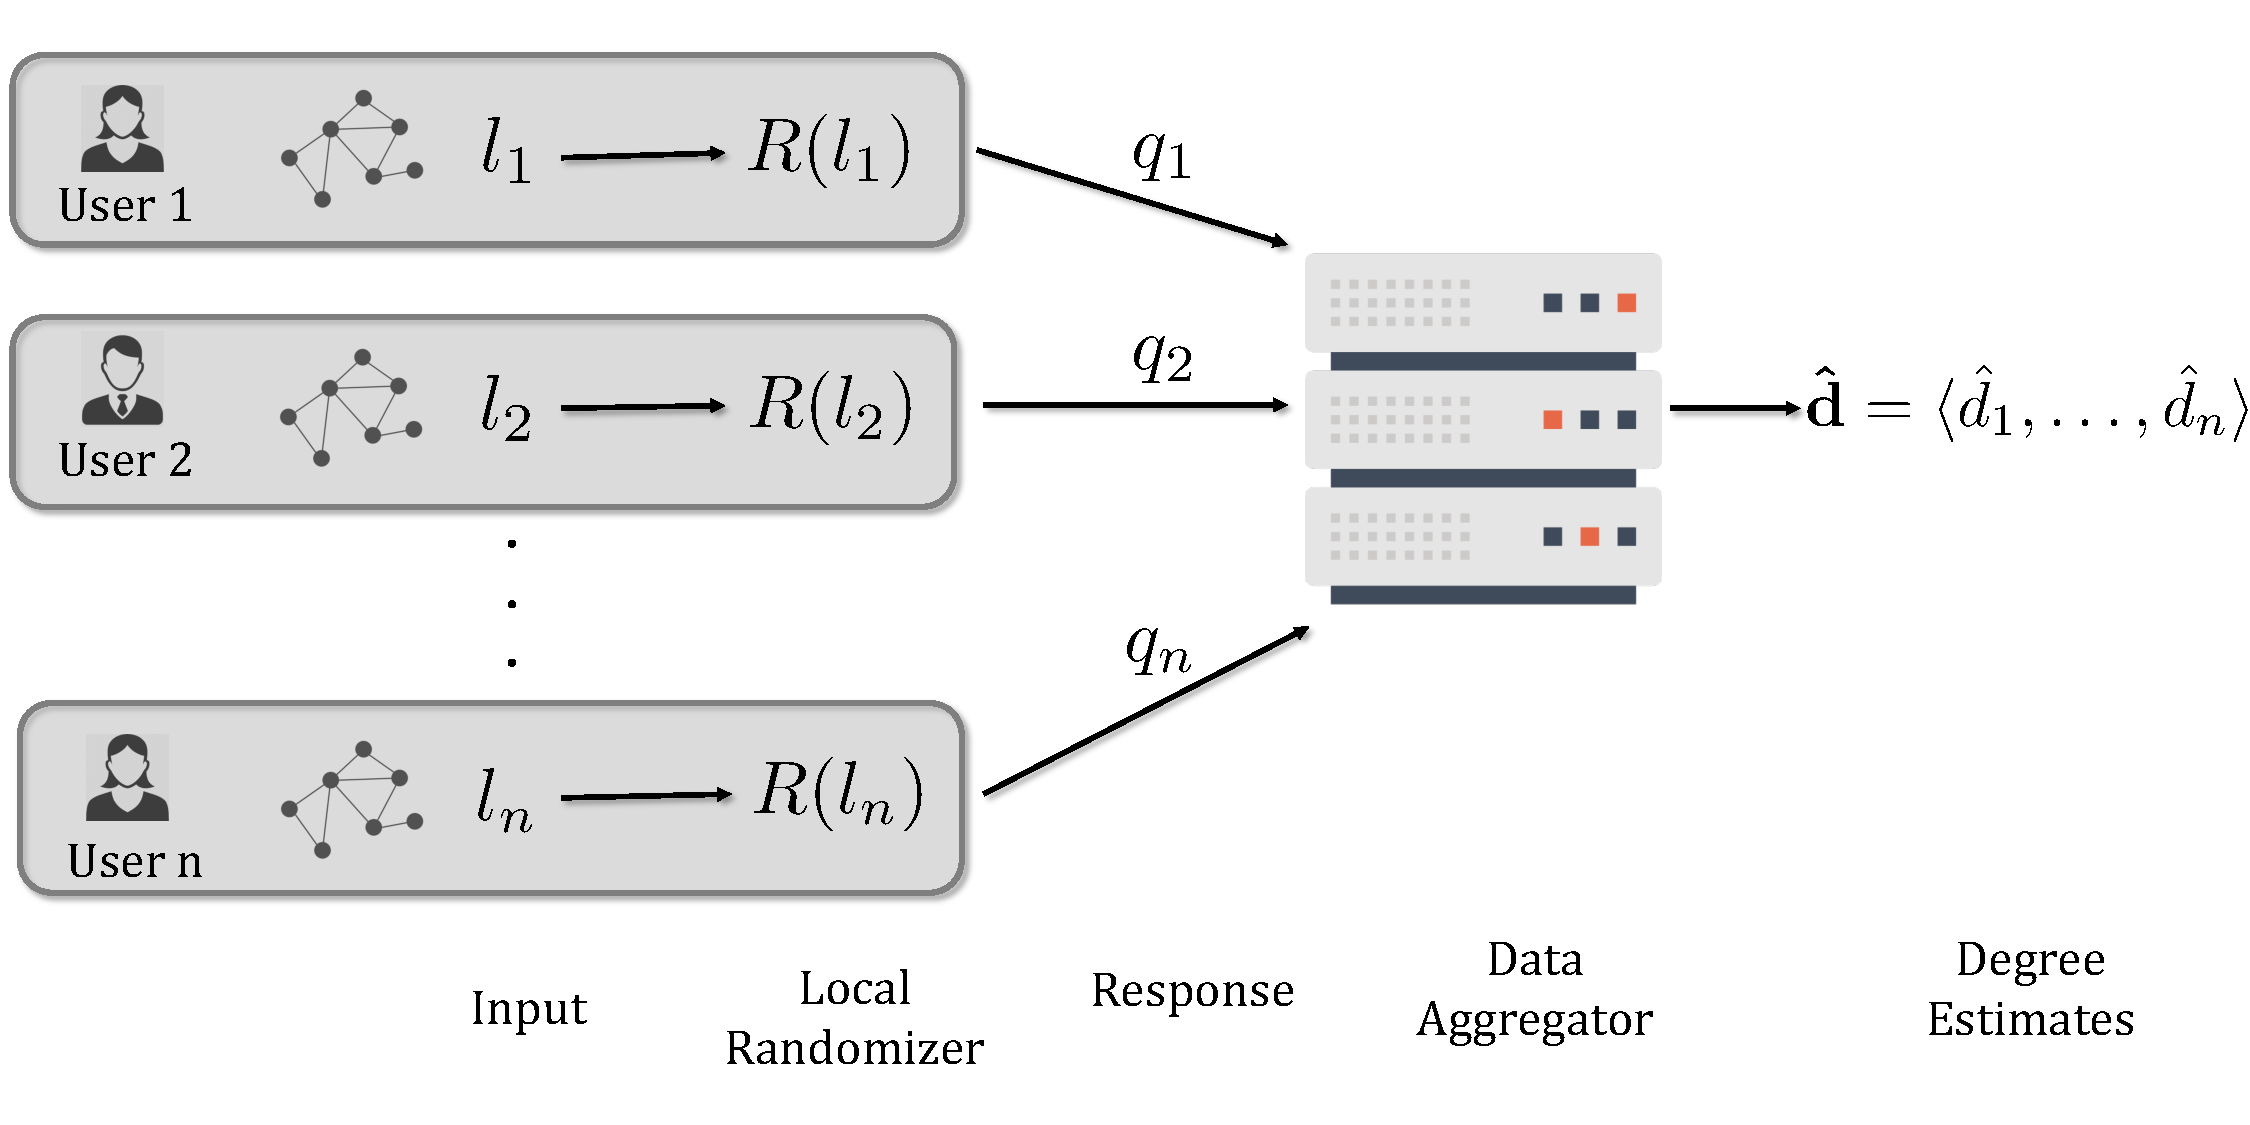
\includegraphics[width=0.78\columnwidth]{graph_pic_1_new.pdf}
     \vspace{-0.3cm}
  \caption{Graph analysis in the \ldp~setting}
    \label{chap4-fig:setting}   
    \vspace{-1cm}
\end{figure}

Prior work, which focuses on tabular data~\cite{Cheu21,Cao_USENIX21,Li22}, finds that  poisoning attacks can be carried out against naive \ldp{} protocols. However, the impact of poisoning under \ldp{} for graph analysis is largely unexplored. In this paper, we initiate a formal study on the impact of such poisoning attacks on \ldp{} protocols for graph statistics. We focus on the task of degree estimation, one of the most fundamental tasks in graph analysis. 

A real-world use-case for a poisoning attack is as follows. Suppose a data analyst is interested in hiring the most influential nodes (users) of a graph for marketing and uses a node's degree as its measure of influence.  Here, an adversary might want to promote a specific malicious node (user) to be selected as an influencer or prevent an honest node from being selected as an influencer. Concretely, suppose a single malicious user wants to (falsely) get themselves selected as the most influential node. If the \ldp~protocol used is the Laplace mechanism, where each user directly submits their (noisy) degree to the analyst (Fig. \ref{chap4-fig:setting}), then the malicious user can lie flagrantly and report their degree to be $n-1$. This can skew the response by as much as the number of users!

%A near-optimal solution to degree-estimation with \ldp~is the Laplace mechanism where every user directly submits their (noisy) degree to the analyst (Figure \ref{chap4-fig:setting}). If this is the pthe malicious user can hack into the mobile application collecting the data and manipulate the response arbitrarily. Consequently, they can flagrantly lie and respond with $n-1$,  



 %Consider a data analyst interested in hiring the most influential user in a graph for marketing. To do so, the analyst asks each node to release their list of friends (edges) privately. Unfortunately, any estimates based on this protocol are susceptible to data poisoning; for example, an adversary might create fake accounts with whom they are friends or lie about being friends with real users. The second attack is particularly devastating --- the adversary could report that he is friends with everyone in the graph! Finally, an adversary may try to reduce an honest user's influence by compromising their friends and reporting no friendship. These attacks are unique to the graph setting, there is no analogue in the \ldp{} literature on tabular data.

We  address this challenge and design degree estimation protocols that are robust to poisoning attacks. Our algorithms are based on the key observation that graph data is naturally redundant -- the information about an edge $e_{ij}$ is shared by both users $\DO_i$ and $\DO_j$. Leveraging this observation, we propose robust protocols based on two new ideas. First, we use \textit{distributed information} -- we collect the information about each edge from \textit{both} users. The second idea is to \textit{verify} -- the data analyst can verify the consistency of the collected information by leveraging its redundancy. Specifically, as long as at least one of $\DO_i$ or $\DO_j$ is honest, the analyst can check for consistency\footnote{For the ease of exposition, we disregard errors due to machine failures.} between the two bits obtained from $\DO_i$ and $\DO_j$ and detect malicious behavior. 

If there are at most $m$ malicious users, then with no privacy, the data analyst could flag malicious users as those with more than $m$ edge inconsistencies in their reported edges since this is beyond a tolerable number of inconsistencies for an honest user. However, \ldp~requires randomization which makes the user's reports probabilistic. Consequently, the aforementioned simple consistency check cannot be applied directly to \ldp~protocols. We mitigate this challenge by proposing edge inconsistency confidence bounds under \ldp~which guarantees detection of malicious users without misclassifying the honest ones. Using our edge consistency checks we design novel degree estimation protocols under \ldp~which are robust to poisoning attacks.

%To this end, we design novel degree estimation protocols that enable a data analyst to employ consistency checks and detect malicious users even under \ldp. 
 

%We observe that \ldp~makes a degree estimation protocol more vulnerable to poisoning -- the impact of poisoning is worse when the adversary can directly poison their (noisy) responses (Fig. \ref{chap4-fig:response}), rather than their input data (Fig. \ref{chap4-fig:input}).  The former utilizes the characteristics of \ldp~while the latter is independent of \ldp.





In summary, we are the \textit{first} to study the impact of poisoning  on \ldp~degree estimation for graphs. Our main contributions are: 
\squishlist
    \item We propose a formal framework for analyzing the robustness of a protocol. %The framework quantifies the impact of poisoning attacks on both honest and malicious   users. 
Specifically, we measure the robustness along two dimensions, \textit{correctness} (for honest users) and \textit{soundness} (for malicious users). Intuitively, good correctness means that the protocol is accurate for honest users, and good soundness means that it can detect/restrict malicious users. %Hence, a protocol which has both properties is robust to poisoning attacks.
\item Based on the proposed framework, we study the impact of poisoning attacks on private degree estimation in the \ldp~setting. The attacks can be classified into two types: $(1)$ input poisoning attacks  where the adversary does not have access to implementation of the \ldp~protocol and can only falsify their input data (Fig. \ref{chap4-fig:input}), and $(2)$ response poisoning attacks where the adversary can tamper with the \ldp~implementation and directly manipulate the (noisy) responses of the \ldp~protocol (Fig. \ref{chap4-fig:response}). The former is independent of \ldp~while the latter utilizes the characteristics of \ldp. We observe that \ldp~makes a degree estimation protocol more vulnerable to poisoning -- the impact of a response poisoning attack can be worse than that of any input poisoning attack. 
\item Leveraging the natural redundancy in graph data, we design robust degree estimation protocols under \ldp~that significantly reduce the impact of adversarial poisoning and compute degree estimates with high accuracy (Table \ref{chap4-tab:results}).
\item We evaluate our proposed robust degree estimation protocols under poisoning attacks on real-world datasets to demonstrate their efficacy in practice. We observe that even a relatively
small number of malicious parties $(m = 1\% )$ can stage significantly damaging poisoning attacks. This demonstrates the
practical threat of such attacks. Nevertheless, our empirical results show that our proposed protocols are
able to thwart poisoning attacks
even with a large number of malicious users $(m = 37.5\%)$.
\squishend



%We focus on the task of degree estimation and propose protocols provide formal robustness guarantees against data poisoning attacks that significantly reduce the impact of poisoning and compute degree estimates with high accuracy. The key observation Leveraging the redundancy in graph data, we design robust degree estimation protocols under \ldp~that significantly reduce the impact of adversarial poisoning and compute degree estimates with high accuracy. Our empirical 
  


%In this paper, we initiate a formal study of the impact of data poisoning on \ldp{} protocols for graph statistics. We focus on the task of degree estimation, one of the most fundamental tasks in graph analysis which can be used to estimate  node influence. We formalize what it means for an \ldp{} graph protocol to be accurate and robust to data poisoning attacks. Specifically, we permit a protocol to flag a malicious user, and robustness means that a malicious user is either flagged or receives an accurate estimate. Consistent with the attacks described above, under our definitions, the naive randomized response protocol is accurate but not robust. 


%\par We observe that data poisoning can significantly skew the results of standard \ldp~protocols. For instance, consider the Laplace mechanism where every user directly submits their (noisy) degree to the analyst (Fig. \ref{chap4-fig:setting}). However, a malicious user can flagrantly lie and respond with $n-1$,  skewing their response by as much as the number of users. We  address this challenge and design robust degree estimation protocols. Our protocols are based on the key observation --   graph data is naturally redundant. Specifically, the presence (or absence) of edge $e_{ij}$ is shared by both users $\DO_i$ and $\DO_j$. This introduces data redundancy which we leverage to provide robustness -- as long as at least one of $\DO_i$ or $\DO_j$ is honest, the analyst can check for consistency between the two bits obtained from $\DO_i$ and $\DO_j$. We illustrate this using the following degree-estimation protocol. For the ease of exposition, we assume no privacy. Consider a protocol where the users send in their (true) adjacency lists. Here for every edge $e_{ij}$, the analyst receives two copies of the same bit from users $\DO_i$ and $\DO_j$ -- in case there is inconsistency\footnote{For the ease of exposition, we disregard errors due to machine failures.} in the two reported bits, the analyst can safely conclude that one party is malicious and act accordingly. Thus, we see that the natural data redundancy in graphs can be leveraged to perform robust data analysis. However, \ldp~requires randomization which makes the user's reports probabilistic. Consequently, the aforementioned simple consistency check cannot be applied to \ldp~protocols.  To this end, we design novel degree estimation protocols that enable a data analyst to employ consistency checks and detect malicious users even under \ldp. Our proposed protocols provide formal robustness guarantees against data poisoning attacks that significantly reduce the impact of poisoning and compute degree estimates with high accuracy. 

\begin{comment}In summary, we make the following contributions:
\squishlist
  \item 
  \item We propose a formal framework for analyzing the robustness of a protocol. The framework quantifies the impact of poisoning attacks on both honest and malicious   users. 
 \item Based on the proposed framework, we study the impact of poisoning attacks on private degree estimation in the \ldp~setting. We observe that \ldp~makes a degree estimation protocol more vulnerable to poisoning -- the impact of poisoning is worse when the adversary can directly poison their (noisy) responses (Figure \ref{chap4-fig:response}), rather than their input data (Figure \ref{chap4-fig:input}).  The former utilizes the characteristics of \ldp~while the latter is independent of \ldp.

 
  
  \item Leveraging the redundancy in graph data, we design robust degree estimation protocols under \ldp~that significantly reduce the impact of adversarial poisoning and compute degree estimates with high accuracy. 
  
    \item We evaluate our proposed robust degree estimation protocols under poisoning attacks on real-world datasets to demonstrate their efficacy in practice. We observe that even with a with a smasll () cab have significantly 
\squishend
\end{comment}
%In our paper, we first propose a formal framework for analyzing the robustnessof an algorithm under an attack. We study the robustness of a naive algorithm for estimating degrees under two common attacks against \ldp{} protocols. 

%Second, utilizing redundancy in graph data, we design protocols protocols utilizing the redundancy in graphs which also satisfy \ldp{}. Our results demonstrate the following:  (1) that adversarial manipulation becomes worse when the adversary is able to manipulate their (noisy) response, rather than their input data, and (2) that it is possible to leverage the redundancy in graph data to significantly reduce adversarial manipulation.In graphs, redundancy may be used to reduce the influence a malicious party has over \ldp{} protocols. If allowed to return $\bottom$ when auser is believed to be adversarial, a protocol is able to limit theadvantage of an adversary to much below what is achieved by naive approaches.

%\ji{ TODO: Table of results}
\begin{table*}
\centering
\begin{tabular}{|c|ccc|ccc|c|}
\hline 
\multirow{2}{*}{Protocol} & \multicolumn{3}{|c|}{Response Poisoning} & \multicolumn{3}{|c|}{Input Poisoning} & \multirow{2}{*}{Privacy Guarantee} \\
& Correctness & Soundness & & Correctness & Soundness & & \\ \hline
\RLap & $(\tO(\frac{1}{\epsilon}), \delta)$ & $(n-1)$-tight& Thm.~\ref{chap4-thm:response:laplace}& $(\tO(\frac{1}{\epsilon}), \delta)$ & $(n-1, \frac{1}{2})$ & Thm.~\ref{chap4-thm:input:laplace} & $\epsilon$-Edge \ldp\\ \hline 
\DegRRNaive & $(\tO(m + \frac{m}{\epsilon} + \frac{\sqrt{n}}{\epsilon}), \delta)$ & $(n-1)$-tight  & Thm.~\ref{chap4-thm:response:naive} & $(\tO(m + \frac{\sqrt{n}}{\epsilon}), \delta)$ & $(n-1, \frac 1 2)$  & Thm.~\ref{chap4-thm:input:naive} & $\epsilon$-Edge \ldp\\ \hline
\DegRRCheck & $(\tO(m + \frac{m}{\epsilon} + \frac{\sqrt{n}}{\epsilon}), \delta)$ & $(\tO(m + \frac{m}{\epsilon} + \frac{\sqrt{n}}{\epsilon}), \delta)$ & Thm.~\ref{chap4-thm:response:check} & $(\tO(m + \frac{\sqrt{n}}{\epsilon}), \delta)$ & $(\tO(m + \frac{\sqrt{n}}{\epsilon}), \delta)$ & Thm.~\ref{chap4-thm:input:check} & $\epsilon$-Edge \ldp\\ \hline
\DegHybrid & $(\tO(\frac{1}{\epsilon}), \delta)$ & $(\tO(m + \frac{m}{\epsilon} + \frac{\sqrt{n}}{\epsilon}), \delta)$ & Thm.~\ref{chap4-thm:response:hybrid} & $(\tO(\frac{1}{\epsilon}), \delta)$ & $(\tO(m + \frac{\sqrt{n}}{\epsilon}), \delta)$ & Thm.~\ref{chap4-thm:input:hybrid} & $\epsilon$-Edge \ldp \\ \hline
\end{tabular}
\caption{Summary of correctness and soundness results in the paper. The $\tilde{O}$ notation asymptotically holds for $\epsilon<1$, and hides factors of $\log \frac{1}{\delta}$. $n-1$-tight  indicates that there exists a worst-case attack that can skew the degree estimates by $n-1$. All the above results are attack-agnostic. }\label{chap4-tab:results}
 \vspace{-0.5cm}
\end{table*}
\section{Preliminaries}\label{chap4-sec:background}
%In this section, we introduce the necessary background on \ldp~for graph analysis followed by .\\\\\noindent
\textbf{Notation.}
Throughout this paper, let $G = (V, E)$ be an undirected 
graph with $V$ and $E$ representing the set of nodes (vertices) and edges, respectively. We assume a graph with $n \in \mathbb{N}$ nodes, i.e., $V = [n]$ where $[n]$ denotes the set $\{1,2,\cdots,n\}$. Let $\calG$ denote the domain of all graphs with $n$ nodes. Each node $i \in V$ corresponds to a user $\DO_i$. Let $l_i \in \{0,1\}^n$ be the adjacency list for $\DO_i, i \in [n]$ where bit $l_i[j], j \in [n]$ encodes the edge $e_{ij}$ between a pair of users $\DO_i$ and $\DO_j$. Specifically, $l_i[j]=1$ if $e_{ij}\in E$ and $e_{ij}=0$ otherwise. %Note that $l_i$ is the $i$-th row of the adjacency matrix $L$ of the graph $G$. 
Let $\textbf{d}=\langle d_1, \ldots, d_n\rangle \in \R^n$ denote the vector of degrees in $G$. $m$ denotes the number of malicious users.


\subsection{Local Differential Privacy for Graphs}\label{chap4-sec:ldp}
%Differential privacy (\DP) is a quantifiable measure of the stability of the output of a randomized mechanism to changes to its input. 
Our paper focuses on the \textit{local} model of \DP, one of the most popular models. % There are two popular models of differential privacy, \textit{local} and \textit{central}.
The local model consists of a set of individual users (\DO) and an untrusted data aggregator (analyst); each user perturbs their data using a (local) \DP~algorithm and sends it to the aggregator which uses these noisy data to estimate certain statistics of the entire dataset. %Thus, the \ldp~model allows gleaning of useful information from the dataset without requiring the data owners to trust any third-party entity. %This makes it an attractive model for commercial deployment~\cite{Apple,Rappor1,Rappor2,Uber}.
  %An edge $e_{ij}$ is shared between two users $\DO_i$ and $\DO_j$. 
 
The most popular privacy guarantee for graphs in the local setting is known as \textit{edge \ldp}~\cite{Graph7,Graph11} which protects the existence of an edge between any two users. In other words, on observing the output, an adversary cannot distinguish between two graphs that differ in a single edge. Formally, we have:
\begin{defn}[$\epsilon$-Edge~\ldp\cite{qin2017generating}]
    Let $R: \{0,1\}^n\mapsto \mathcal{X}$ be a randomized algorithm that takes an adajcency list $l \in \{0,1\}^n$
as input. We say $R(\cdot)$ provides $\epsilon$-edge LDP if for any two
neighboring lists $l,l' \in \{0,1\}^
n$ that differ in one bit (i.e., one
edge) and any output $s \in \mathcal{X}$,\vspace{-0.3cm}
\begin{gather} \mathrm{Pr}
[R(l) = s]\leq e^{\epsilon}\mathrm{Pr}[R(l') = s]
\end{gather}
\end{defn}
 


\begin{comment}As noted above, the knowledge of an edge in a graph is shared between two users. Motivated by this observation, recent work~\cite{imola2021locally,imola_communication-efficient_2022} has introduced a new notion of \DP~called relationship \DP~that considers both the users' outputs and \textit{hides an edge in a graph during the entire computation}. Formally, we have:
\begin{defn}[$\epsilon$-relationship \DP]  For $i \in [n]$,
let $R_i: \{0,1\}^n\mapsto \calX$ be the local randomizer of user $\DO_i$ that takes their adjacency list $l_i$ as input.
We say $\langle R_1(\cdot),\cdots,R_n(\cdot)\rangle$ provides $\epsilon$-relationship \DP~if for any
two neighboring graphs $G,G' \in \calG$ that differ in one edge and
for any $S\subseteq \calX^n$,
\begin{multline*}
\Pr[(R_1(l_1),\cdots,R_n(l_n)) = S]
\leq e^{\epsilon} \Pr[(R_1(l'_1),\cdots,R_n(l'_n))=S], \end{multline*}
where $l_i$ (respectively, $l_i'$)
is the $i$-th row of the adjacency
matrix of graph $G$ (respectively, $G'$).\end{defn}

Relationship \DP~is closely connected to the notion of edge \ldp~which is one of the most popular privacy guarantee for graphs \cite{Graph7,Graph11} in the \ldp~setting. 
$\epsilon$-edge \ldp~protects the information about an edge $e_{ij}$ from the adjacency list $l_i$ of a \textit{single} user $\DO_i$. On the other hand, relationship \DP~consider the outputs from \textit{both} users $\DO_i$ and $\DO_j$ and hides the \textit{edge as a  whole}. Formally, if each of the local randomizers $R_i(\cdot), i \in [n]$ satisfy $\epsilon$-edge \ldp, then $\langle R_1(\cdot),\cdots,R_n(\cdot)\rangle$ satisfies $2\epsilon$-relationship \DP~\cite{Graph7,Graph11}. Next, we describe two common privacy mechanisms for degree estimation.
% For the rest of the paper, we consider $\epsilon$-relationship \DP~degree estimation algorithms.
\end{comment}


%Two adajacency lists are defined to neighboring lists if 
\noindent\textbf{Randomized Response.} Randomized Response ($RR_\rho(\cdot)$)~\cite{RR} releases a bit $b \in \{0,1\}$ by
flipping it with probability $\rho = \frac{1}{1+e^\epsilon}$. We extend the
mechanism to inputs in $\{0,1\}^n$ by flipping each bit independently with
probability $\rho$ (Alg.~\ref{chap4-alg:rr} in App. \ref{chap4-app:background}) which satisfies
 $\epsilon$-edge \DP. 
 
\noindent\textbf{Laplace Mechanism.} 
The Laplace mechanism(\RLap) is a standard algorithm to achieve \DP~\cite{Dwork}. For degree estimation, each user $\DO_i$ simply reports $\tilde{d}_i=d_i+\eta, \eta \sim Lap(\frac{1}{\epsilon})$ where $Lap(b)$ represents the Laplace distribution with scale parameter $b$. This mechanism satisfies $\epsilon$-edge \DP. 

Every protocol used in this paper is based on randomized response, the Laplace mechanism, or a composition thereof, and it is easy to show each one satisfies $\epsilon$-edge LDP.

\subsection{Protocol Setup}
\noindent\textbf{Problem Statement.}  
We consider single round,  non-interactive protocols in which each user $\DO_i, i \in [n]$ runs the local randomizer
$R_i : \{0,1\}^n \rightarrow \calX$ for some output space $\calX$ on their adjacency lists $l_i$ (Fig. \ref{chap4-fig:setting}). The data aggregator collects the noisy responses and applies a function 
$D : \calX^n \rightarrow (\mathbb{N} \cup \{\bottom\})^d$ to produce final degree estimates  $\hat{\textbf{d}}=\langle \hd_1, \ldots, \hd_n\rangle)$. Here, $\hd_i$ is the aggregator's estimate for $d_i$ for user $\DO_i$. Note that the aggregator is allowed to output a special symbol $\bottom$ for a user $\DO_i$ if they believe the estimate $\hat{d}_i$ to be invalid (i.e., $\DO_i$ is malicious).
  \vspace{-0.2cm}  \\\\
\noindent\textbf{Threat Model.}
In the execution of a protocol $\calP$, a subset of users $\calM \in [n]$ may be malicious. The malicious users may return arbitrary output with the goal of carrying out a poisoning attack on  $\calP$. Let
$m=|\calM|$ denote the number of malicious users. We refer to 
$\calH = [n] \setminus \calM$ as the set of honest users.
We do not make any assumptions on how the malicious users are instantiated in practice -- they could correspond to either fake accounts created by the adversary or a set of real accounts which have been compromised or a combination of both. 

Based on the specifications of the practical implementation of the \ldp, there is an important distinction between the way in which the malicious users may carry out their poisoning attacks. We outline them as follows:

\squishlist
    \item \textbf{Input Poisoning.} In this threat model, the users do not have access to the implementation of the \ldp{} randomizer. For instance, mobile applications might run proprietary code which the users do not have permission to tamper with. Consequently, the only thing a malicious user can do is falsify their underlying input data, i.e.,  change their input from $l_i$ to an arbitrary $l_i'$, and then report $q_i = R_i(l_i')$ (Fig. \ref{chap4-fig:input}).
    
    \item \textbf{Response Poisoning.} This is a stronger threat model where a malicious user has direct control over the implementation of the \ldp{} randomizer. For instance, the user could hack into the mobile application collecting their data. Consequently, the user can completely bypass the randomizer and submit an arbitrary response $q_{i}$ (Fig. \ref{chap4-fig:response}) to the aggregator.
\squishend

Note that input poisoning attack applies to \textit{any} protocol, private or not, because a user is free to change their input anytime. However, response poisoning attacks are unique to \ldp{} -- the distinction between an user's input and their response is a characteristic of \ldp{} which we results in a separation in the efficacy of the two types of attacks (see Sec. \ref{chap4-sec:input-attacks} for details). 


\begin{figure}
    \vspace{-0.5cm}
    \centering
    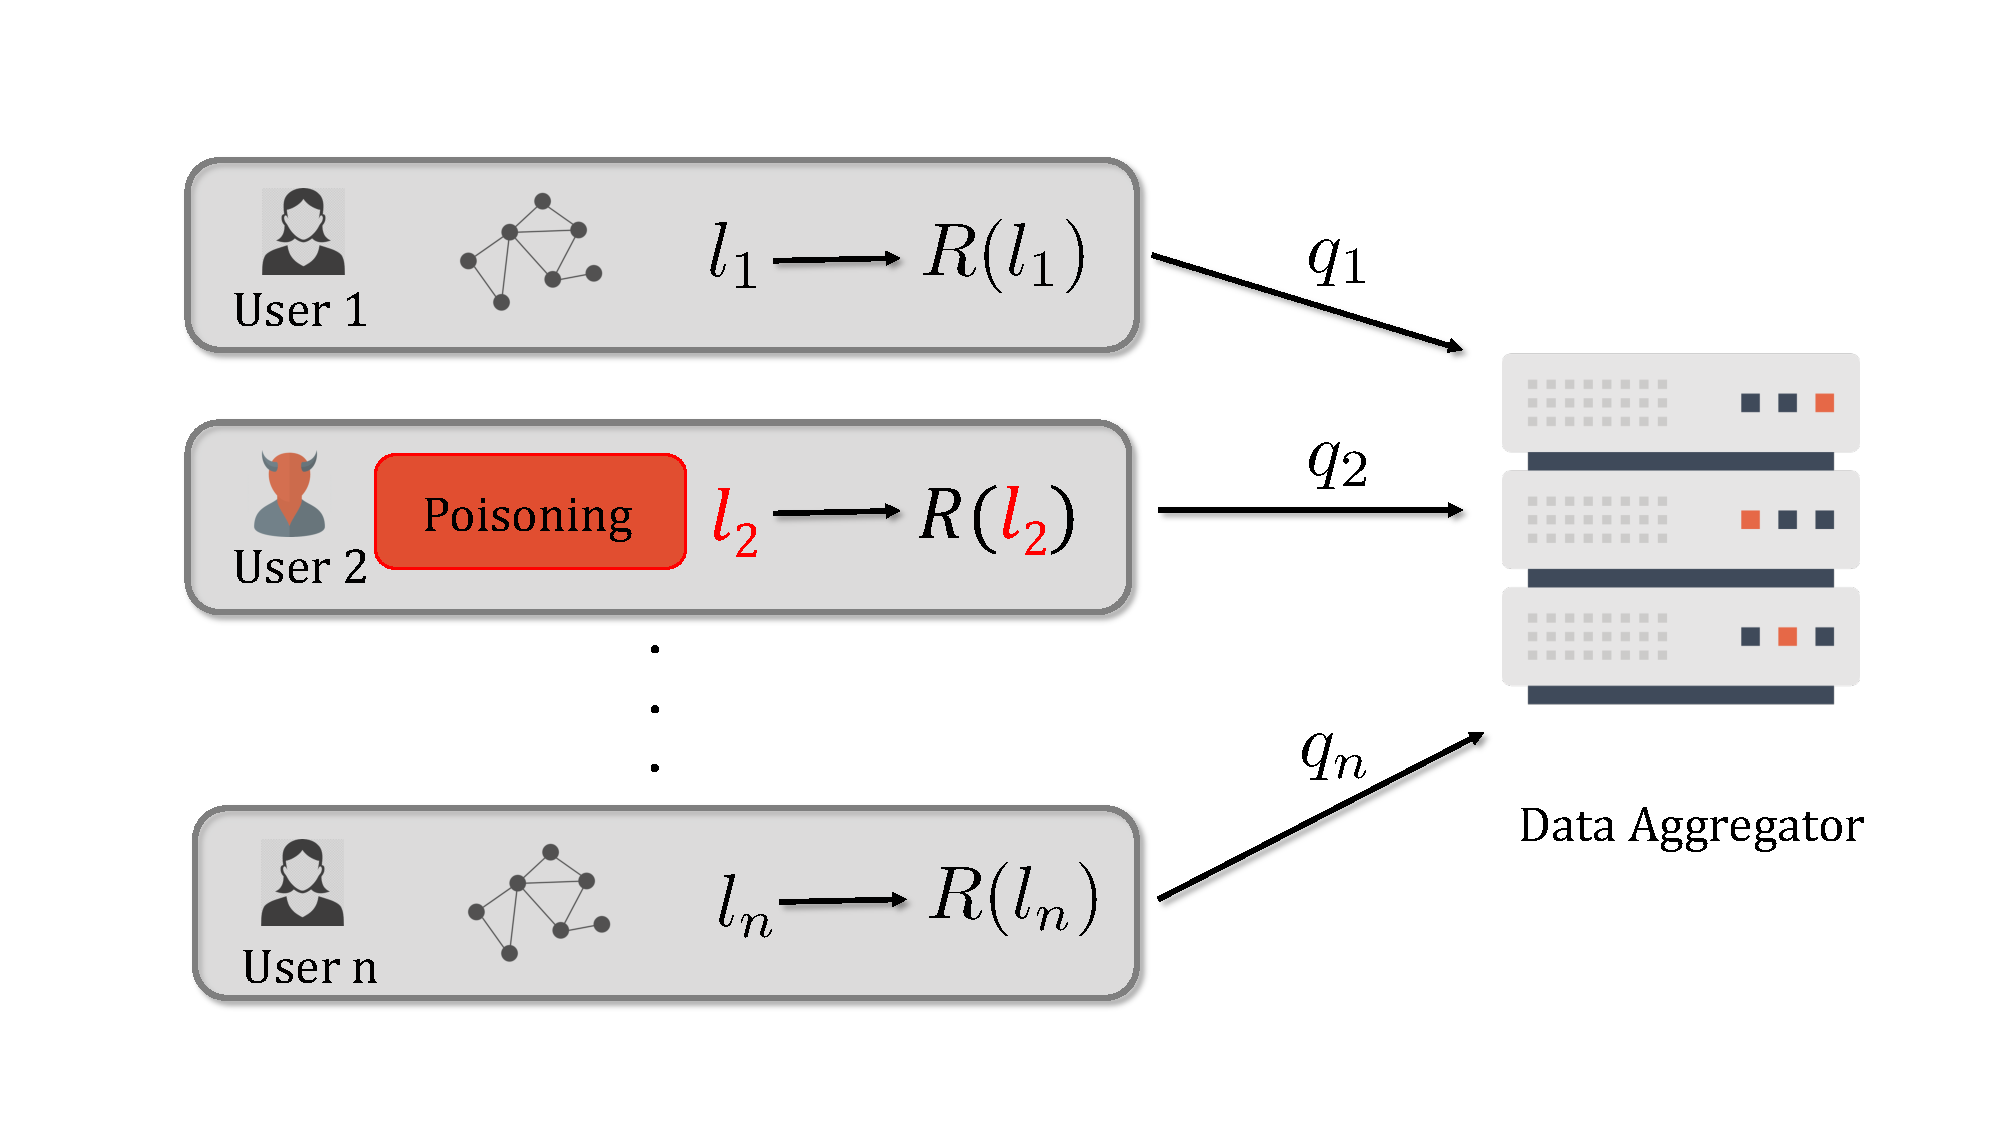
\includegraphics[width=0.8\columnwidth]{graph_pic_3.pdf}
    \vspace{-0.5cm}
    \caption{Input Poisoning Attack}
    \label{chap4-fig:input} 
        \vspace{-0.6cm}
\end{figure}
\begin{figure}[bt]
    \centering
 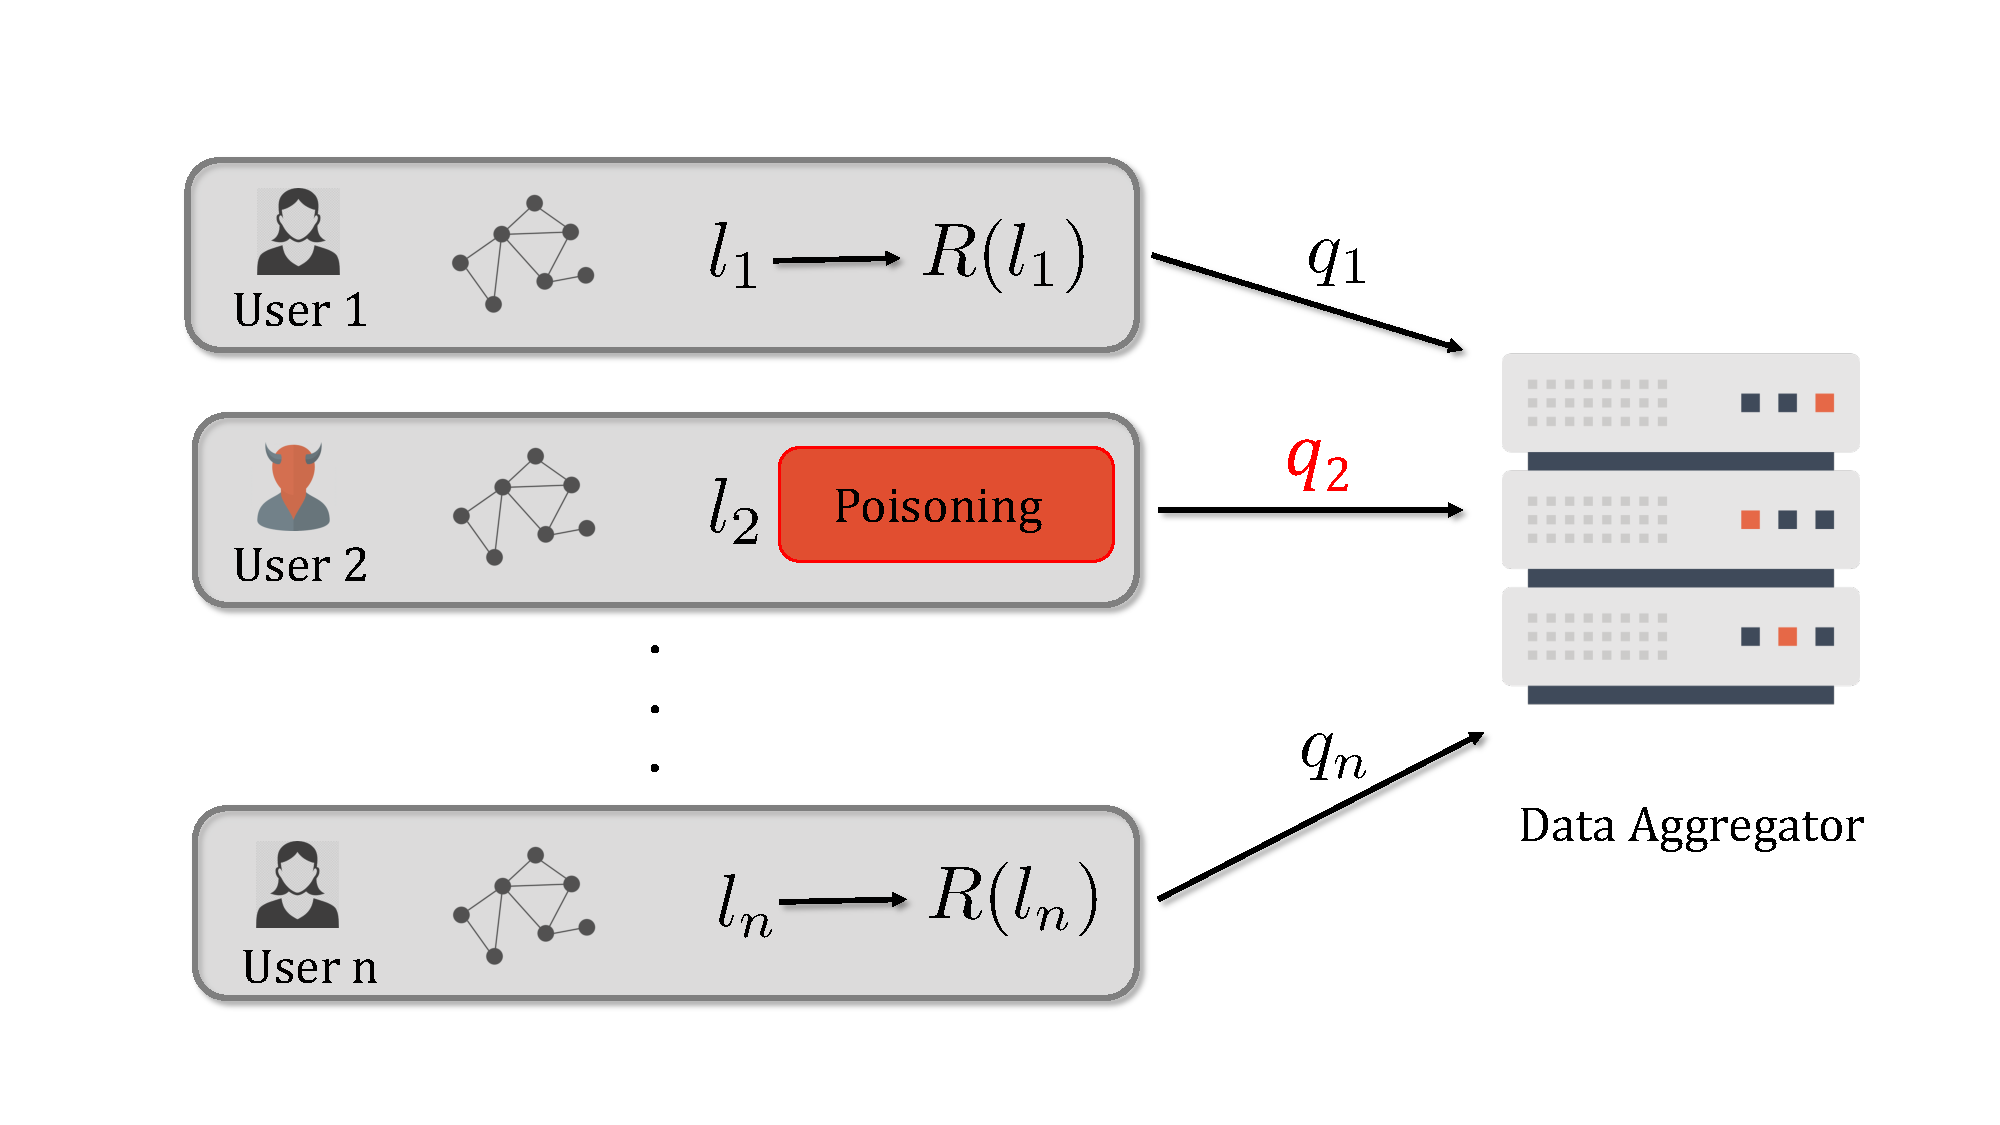
\includegraphics[width=0.8\columnwidth]{graph_pic_2.pdf}
     \vspace{-0.5cm}
   \caption{Response Poisoning Attack}
    \label{chap4-fig:response} \vspace{-0.5cm}
\end{figure}





  \vspace{-0.2cm}  \subsection{Motivating Attacks}\label{chap4-sec:attacks}

For the Laplace mechanism, \RLap, and randomized response mechanism, $RR_\rho$,  outlined in Sec.~\ref{chap4-sec:ldp}, we present two concrete motivating attacks. We consider the attacks in the context of the task of influential node identification, where the goal of the data aggregator is to identify certain nodes with a high measure of ``influence". This is useful for various applications where the influential nodes are selected for disseminating information/advertisement. Here, we consider the simplest measure of influence -- degree; nodes with the top-$k$ degrees are selected as the influencers. With the goal of modifying the influence of different users, a malicious user may choose to carry out the following attacks:
  \vspace{-0.2cm}  \\\\\noindent\textbf{Degree Inflation Attack.} In this attack, a target malicious user $\DO_t$ wants to get themselves selected as an influential node. For \RLap, since each user sends their degree $d_i$ plus Laplace noise, the target user maximizes their degree estimate by simply sending $n-1$. 

For $RR_\rho$, the target malicious user $\DO_t$ colludes with a set of other users  (for instance, by injecting fake users) as follows. All the non-target malicious users $\DO_i, i \in \calM\setminus t$ report $1$ for the edges corresponding to $\DO_t$. Additionally, $\DO_t$ reports an all-one list.   \vspace{-0.2cm}  \\\\
\noindent\textbf{Degree Deflation Attack.}   In this attack, the target is an honest user $\DO_t \in \calH$ who is being victimized by a set of malicious users (for instance, the adversary compromises a set of real accounts with an edge to $\DO_t$) -- $\calM$ wants to ensure that $\DO_t$ is \textit{not} selected as an influential node. The attack strategy is to decrease the aggregator's degree estimate $\hd_t$ for $\DO_t$. For \RLap, there is no way for the malicious party to influence $\hd_t$. However, for randomized response, the malicious users may report $0$ for each edge in $\calM$ connected to $\DO_t$, reducing their degree by this amount. %\ji{We might be able to improve degree deflation attacks!}


\section{Quantifying Robustness}\label{chap4-sec:framework}

In this section, we present our formal framework for analyzing the robustness of a protocol for degree estimation. Specifically, we measure the robustness along two dimensions, \textit{correctness} (for honest users) and \textit{soundness} (for malicious users). Intuitively, good correctness means that the protocol is accurate for honest users, and good soundness means that it can detect/restrict malicious users. Hence, a protocol which has both properties is robust to poisoning attacks. %To the best of our knowledge, we are the first to analyze the correctness and soundness to \ldp~protocols for graphs. \ji{Is this right/adequate?}


\subsection{Metrics}\label{chap4-sec:robustframework}

%In order to achieve robustness, we permit our algorithms to return $\hat{d}_i = \bottom$ (abort the estimate for user $\DO_i$) if it detects poisoning in that user's data. The symbol $\bottom$ means that the data received about $\DO_i$ does not constitute a valid input and their degree estimate is aborted. 
Our notion of correctness guarantees that the protocol will produce an accurate degree estimate $\hat{d}_i$ for an honest user $\DO_i \in \mathcal{H}$ even under poisoning. On the other hand, good soundness prevents a malicious user $\DO_i \in \calM$ from  manipulating their degree estimate by too much \textit{without} detection.   We describe them in details as follows.  \vspace{-0.2cm}  
\\\\
\noindent\textbf{Correctness (For Honest Users).}
The \textit{correctness} of a protocol assesses its resilience to manipulation of an honest user's estimator. Specifically,  malicious users can adversely affect an honest user $\DO_i \in \calH$ by \squishlist\item tampering with the value of $\DO_i$'s degree estimate $\hat{d}_i$ (by introducing additional error), or \item attempting to mislabel $\DO_i$ as malicious (by influencing the aggregator to report $\hat{d}_i=\bot$) \squishend
Correctness protects the honest user $\DO_i$ along the above dimensions and is formally defined as follows:


\begin{defn}\label{chap4-def:correct}(\textbf{Correctness}) Let 
  $\langle R_1, \ldots, R_n\rangle$ be a non-interactive, \ldp{} protocol for degree estimation producing estimates $\langle \hd_1, \ldots, \hd_n\rangle$. Let $\calM$ be a set of malicious users with $|\calM| = m$ and $\calH$ be the set of honest users. 
Then, the protocol is defined to be $(\alpha_1,\delta_1)$-correct w.r.t. an attack from $\calM$ if for all input graphs $G\in \calG$ we have:
  \begin{gather}  \vspace{-0.2cm}  
    \forall \DO_i \in \calH, \mathrm{Pr}\left[\hat{d}_i = \bottom \vee
    |\hat{d}_i-d_i|\geq \alpha_1\right]\leq \delta_1,\label{chap4-eq:correct1}
  \end{gather}
where the above probability is taken w.r.t  the randomness in the protocol and the attack.
\end{defn}
The parameter $\alpha_1$ dictates the accuracy of the estimate $\hat{d}_i$, and the parameter $\delta_1$ dictates the chance of failure---that either of the aforementioned conditions fail to hold. Thus, if a protocol is $(\alpha_1,\delta_1)$-correct, it means that with probability at least $(1-\delta_1)$, 
the degree estimate $\hd_i$ for any honest user $\DO_i \in \calH$ has error \textit{at most} $\alpha_1$, \textit{and} $\DO_i$ is guaranteed to be \textit{not} mislabeled as malicious.

Complementary to the above definition, we introduce the notion of $\alpha_1$-\textit{tight correctness}. A protocol is defined to be $\alpha_1$-tight correct w.r.t an attack, if there exists a graph such that the attack is \textit{guaranteed} to either skew the  the degree estimate of at least one honest user by \textit{exactly} $\alpha_1$.  We use this definition to show the existence of strong attacks that are guaranteed to be very successful in manipulating the data of an honest user, which motivates the need for robust solutions. 

Lower the value of
$\alpha_1$ and $\delta_1$, better is the robustness of the protocol for honest users.  \vspace{-0.2cm}  \\\\ 
%This definition is the complement of Definition~\ref{chap4-def:correct}, and we use it to show that there are attacks which, in a strong sense, are very successful against the protocol: They are always able to return $\bottom$ or an inaccurate response for an honest user. We use this definition to motivate the need for more robust algorithms.\\\\
\noindent\textbf{Soundness (For Malicious Users). } The \textit{soundness} of a protocol assesses its ability to restrict adversarial manipulations of a malicious user's estimator. In particular, the protocol either returns an accurate estimate or returns $\hd_i = \bottom$ for these malicious users, regardless of the poisoning attack used. Formally, we use the following definition (which uses the complement event $\hd_i \neq \bottom \wedge |\hd_i - d_i| \geq \alpha_2$):

\begin{defn}\label{chap4-def:sound}(\textbf{Soundness}) Let $\langle R_1, \ldots, R_n\rangle$ be a non-interactive, \ldp{} protocol for degree estimation producing estimates $\hd_1, \ldots, \hd_n$. Let $\calM$ be a set of malicious users with $|\calM| = m$ and $\calH$ be the complement set of honest users. Then, the protocol is defined to be $(\alpha_2, \delta_2)$-sound w.r.t an attack from $\calM$ if, for all input graphs $G \in \calG$ we have
  \begin{gather}
    \forall \DO_i \in \calM, \mathrm{Pr}\left[\hd_i \neq \bottom \wedge |\hd_i -
    d_i| \geq \alpha_2\right]\leq \delta_2, \label{chap4-eq:sound1}
  \end{gather}
  where the above probability is taken w.r.t randomness in the protocol and attack.
\end{defn}
Like with correctness, the parameter $\alpha_2$ dictates the accuracy of the estimate $\hat{d}_i$, and $\delta_2$ dictates the chance of failure. As an important distinction, note that the failure event is when $\hat{d}_i$ is both $\neq \bottom$ \textit{and} is inaccurate, as stated above. Thus, the $\vee$ used in the definition of correctness is replaced by a $\wedge$. In other words, a protocol is $(\alpha_2,\delta_2)$-sound if for any malicious user $\DO_i, i \in \calM$, the protocol \squishlist \item fails to identify $\DO_i$ as malicious, \textit{and} \item reports its degree estimate $\hd_i$ with error \textit{greater} than $\alpha_2$ \squishend  with probability at most $\delta_2$.

Complementary to the above definition, we introduce the notion of $\alpha_1$-\textit{tight soundness}. A protocol is defined to be $\alpha_1$-tight sound w.r.t an attack if there exists a graph $G \in \calG$ such that at least one malicious user is \textit{guaranteed} to have their degree estimate misestimated by \textit{exactly} $\alpha_1$ \textit{without} getting detected.  %This is especially important in our context since every attack is trivially  $(n-1,1)$\footnote{We do not consider self-edges or loops in the graph.}-correct/sound. 
In other words, an $(n-1)$-tight sound/correct attack represents the strongest possible attack\footnote{We do not consider self-edges or loops in the graph.} -- an user's estimate can \textit{always} be skewed by the worst-case amount. We use this definition to motivate the need for more robust protocols. %Note that this is distinct from $(n-1,1)$ correct/sound which is trivial because all events occur with probability $<1$.
\par Lower the value of
$\alpha_2$ and lower the value of $\delta_2$, better is the robustness of the protocol for malicious users.  
  \vspace{-0.2cm}  \\\\
\noindent\textbf{Note.} Our proposed  framework strives to provide a strong notion of robustness -- not only are we able to guarantee accurate estimates, but also detect  \textit{and} flag individual malicious users (by reporting $\bottom$). %This is analogous to the guaranteed output delivery (GOD) model of security multi-party computation in cryptography~\cite{} which is the strongest security model.
%\arc{Expand on this}
\section{Impact of Poisoning on Baseline Protocols}

Within our robustness framework, we analyze the two naive private mechanisms outlined in Sec.~\ref{chap4-sec:ldp} -- the Laplace mechanism and randomized response. The shortcomings of these mechanisms motivate the design of our robust protocols discussed later in the paper. We present all our results for the stronger threat model of response poisoning attacks first. We defer all our discussion for the input poisoning attack to Sec. \ref{chap4-sec:input-attacks}. 

\subsection{Laplace Mechanism}

The simplest mechanism for estimating an user's degree is the Laplace mechanism, \RLap. Recall here, each user directly reports their noisy estimates. Consequently, the degree estimate of an honest user \textit{cannot} be tampered with at all -- the $\tilde{O}(\frac{1}{\epsilon})$\footnote{$\tilde{O}$ hides factors of $\log\frac{1}{\delta}$ } term is due to the error of the added Laplace noise. This error is in fact optimal (matches that of central \DP) for degree estimation.  On the flip side, a malicious user can flagrantly lie about their estimate without detection resulting in the the worst-case soundness guarantee. Specifically,  there
exists a graph and an attack against \RLap{} in
which a malicious user is guaranteed to manipulate their true degree by $n -1$ --
this holds for the case where the malicious user is an isolated node but
lies that their degree is $n - 1$. The robustness of \RLap{} against response poisoning attacks is formalized as follows: 
\begin{thm}\label{chap4-thm:response:laplace}
	Let $\calM$ be a set of malicious users with $|\calM| = m$. The \RLap{} protocol is $(\frac{1}{\epsilon}\log\frac{n}{\delta}),\delta)$-correct with respect to any response poisoning attack from $\calM$. However, there is a response poisoning attack $\calA$ such that \RLap{} is $(n-1)$-tight sound with respect to $\calA$.
\end{thm}
The proof of the above theorem is in App. \ref{chap4-app:thm:response:laplace}.
Thus according to our robustness framework, \RLap{} has good correctness but not soundness. Intuitively, \RLap{} fails to provide good soundness because there is no way to verify the malicious users' reports. 
It is important to note that  \RLap{} has good correctness guarantee even with $n-1$ malicious users while the worst-case soundness is inevitable even with a single malicious user. 
\subsection{Randomized Response}\label{chap4-sec:protocol:naive}
In this section, we look at an alternative mechanism where the users release their edges via randomized response. Recall that the information about an edge is shared between two users -- the idea here is to leverage this \textit{distributed information}. For our baseline algorithm, \DegRRNaive~(described in Alg.~\ref{chap4-alg:degrrnaive}), the data aggregator collects information about an edge from a \textit{single} user. Specifically, for edge $(i,j)$ with $i < j$, it simply uses the response from user $\DO_i$ to decide if the edge exists. To estimate the degree, it counts the total number of edges to user $\DO_i$ with the random variable $count_i^1$ and then computes a debiased estimate of the degree. Note that this naive approach is used by many prior works in local graph algorithms, such as~\cite{LDPGraph1, LDPGraph2,imola2021locally,imola_communication-efficient_2022}.
\setlength{\textfloatsep}{4pt}

\begin{algorithm}[t]
	\SetAlgoLined
  \KwData{$\{l_1,\cdots,l_n\}$ where $l_i \in \{0,1\}^n$ is the adjacency list of user $\DO_i$}
  \KwResult{$(\hat{d}_1,\cdots, \hat{d}_n)$ where $\hat{d}_i$ is the degree estimate for user $\DO_i$}
	
	\textbf{Users}\;
	\ForEach{$i \in [n]$}{
		$q_i = \rr_\rho(l_i)$\;
	}
	\textbf{Data Aggregator:}
	\ForEach{$i \in [n]$}{
    $count_i^1 = \sum_{j < i} q_j[i] + \sum_{i < j} q_i[j]$\;
    $\hd_i = \frac{1}{1-2\rho}(count^1_i - \rho (n-1))$\;
	}
\KwRet{$(\hd_1, \hd_2, \ldots, \hd_n)$}
\caption{\DegRRNaive$: \{0,1\}^{n\times n}\mapsto \{\mathbb{N}\cup \{\bot\}\}^n$}\label{chap4-alg:degrrnaive}

\end{algorithm}


% \begin{algorithm}
%  \caption{\DegRRNaive$: \{0,1\}^{n\times n}\mapsto \{\mathbb{N}\cup \{\bot\}\}^n$}\label{chap4-alg:degrrnaive}
%  \begin{algorithmic}[1]
%  \Statex \textbf{Parameter:} $\epsilon$ - Privacy parameter
%  \Statex \textbf{Input:} $\{l_1,\cdots,l_n\}$ where $l_i \in \{0,1\}^n$ is the adjacency \Statex \hspace{1.2cm} list of user $\DO_i$;
%  \Statex \textbf{Output:} $(\hat{d}_1,\cdots, \hat{d}_n)$ where $\hat{d}_i$ is the degree estimate for  \Statex \hspace{1.2cm} user $\DO_i$;
%  \Statex \textbf{Users}
%    \For{$i \in [n]$}
%      \State $q_i = \rr_\rho(l_i)$
%    \EndFor

%    \Statex \textbf{Data Aggregator}
%    \For{$i \in [n]$}
%      \State $count_i^1 = \sum_{j < i} q_j[i] + \sum_{i < j} q_i[j]$
%      \State $\hd_i = \frac{1}{1-2\rho}(count^1_i - \rho (n-1))$
%    \EndFor
%    \Return $(\hd_1, \hd_2, \ldots, \hd_n)$ 
% \end{algorithmic}
%\end{algorithm}

Formally
for response poisoning attacks, we have:
\begin{thm}\label{chap4-thm:b3a2_hard} 
Let $\calM$ be a set of malicious users with $|\calM| = m$. Then, 
the \DegRRNaive{} protocol is $(m\frac{e^\epsilon+1}{e^\epsilon-1}+\sqrt{n}\frac{\sqrt{(e^\epsilon+1)\ln\frac{2n}{\delta}}}{e^\epsilon-1},\delta)$-correct with respect to any response poisoning attack from $\calM$. However, there is a response poisoning attack $\calA$ such that \DegRRNaive{} is $(n-1)$-tight sound with respect to $\calA$.
\label{chap4-thm:response:naive}\end{thm}
The above theorem is proved in App. \ref{chap4-app:thm:response:naive}.
For $\epsilon < 1$, the correctness guarantee is $\approx m(1+\frac{1}{\epsilon})+\frac{\sqrt{n}}{\epsilon}$. Intuitively, the $\frac{\sqrt{n}}{\epsilon}$ term comes from the error introduced by randomized response. The $m(1+\frac{1}{\epsilon})$ term comes from the adversarial behavior of the malicious users -- $m$ term is inevitable and 
 accounts for the worst case scenario where all $m$ malicious users are colluding  (see Sec. \ref{chap4-sec:discussion}  for more details), while the $\frac{1}{\epsilon}$ factor corresponds to the scaling factor required for de-biasing. This observation is in line with prior work \cite{Cheu21} that assesses the impact of poisoning attacks on tabular data.  Clearly, smaller the value of $\epsilon$, worse is the impact of the attack.   %  who can carry out an increasingly strong attack with smaller $\epsilon$ since they can deterministically report $0$s for the edges to user $i$, not following randomized response which would dictate that $0$ or $1$ is returned with probability close to $\frac{1}{2}$. This harms the debiasing step used to compute $\hat{d}_i$.  %We will more completely discuss this phenomenon in later sections.


Similar to the Laplace mechanism, \DegRRNaive{} is $(n-1)$-tight sound, i.e., a malicious user can always get away with the worst-case $n-1$ error. This happens when $\DO_n$ is an isolated node who acts maliciously and reports an all-one list. Thus, once again this  worst-case soundness is inevitable even with a single malicious user.   In the next section, we discuss how to leverage the data redundancy in graphs and verify the data collected via randomized response to improve the soundness.

%\arc{Motivate what we do next} 


%As each edge is shared by two users, the edge information collected will contain two copies of the edge, one from each user. To decide whether to count an edge or not, our baseline  will simply take the edge information from one user. 


\section{Improving Soundness with Verification}\label{chap4-sec:robust-rr-checks}
%\ji{TODO: clean up theorems and symmetrize them.}

In this section, we present our proposed protocol for robust degree estimation. 
As discussed in the previous section, the naive \DegRRNaive{} protocol offers poor soundness. To tackle
this, we propose a new protocol, \DegRRCheck, that enhances
\DegRRNaive{} with a consistency check based on the
redundancy in graph data and flags users if they fail the check. Consequently, \DegRRNaive{} improves the soundness guarantee significantly. We observe that with higher privacy (lower $\epsilon$), the protocol is less robust. We conclude this section by analyzing \DegRRCheck{} under no privacy constraint---the difference between the correctness and soundness guarantees are the \emph{price of privacy}.

  \vspace{-0.1cm}  \subsection{\DegRRCheck{} Protocol} \label{chap4-sec:protocol:check} 
The \DegRRCheck{} protocol is described in Alg.~\ref{chap4-alg:degrrcheck} and works as follows. \DegRRCheck{} enhances the data collected by \DegRRNaive{} with verification -- for edge $e_{ij} \in E$, instead of collecting a noisy response from just one of the users
$\DO_i$ or $\DO_j$, $\DegRRCheck{}$ collects a noisy response from \emph{both} users. This creates
data redundancy which can then be checked for consistency. Specifically, the estimator counts only those edges $e_{ij}$ for which \textit{both} $\DO_i$ and $\DO_j$ are consistent and report a $1$. 
 The count of noisy edges involving user $\DO_i$ is then given by:
\[count_i^{11} = \sum_{j\in [n]\setminus i} q_{i}[j] q_{j}[i].\]
The unbiased degree estimate of $\DO_i$ is computed as follows:
\begin{equation}\label{chap4-eq:deg-est}\vspace{-0.1cm}
    \hd_i = \frac{count_i^{11} - \rho^2(n-1)}{1-2\rho}.
\end{equation}
%Thus, the degree estimators only count edges for which both users are consistent and report a $1$.


For robustness, \DegRRCheck{} imposes a check on the number of instances of
inconsistent reporting ($\DO_i$ and $\DO_j$ differ in their respective bits reported for their mutual
edge $e_{ij}$). For every user $\DO_i$,  the protocol has an
additional capability of returning $\bot$ whenever the  consistency check fails, indicating
that the aggregator believes that user $\DO_i$ is malicious. The intuition is that if the user $\DO_i$ is malicious and attempts to poison a lot of the edges, then there would be a large number of inconsistent reports corresponding to the edges to honest users. \DegRRCheck{}  counts the number of inconsistent reports for user $\DO_i$ as: 
\[
  count_i^{01} = \sum_{j=1}^n (1-q_{i}[j]) q_{j}[i],
\]
i.e., the number of edges connected to user $\DO_i$\footnote{It is symmetric (and doesn't give additional information) to count edges for which user $\DO_i$ reports $1$ and $\DO_j$ reports $0$.} for
which they reported $0$ and user $\DO_j$ reported $1$. Intuitively, the check computes the expected number of inconsistent reports assuming user $\DO_i$ to be honest and flags $\DO_i$ in case the reported number is outside a confidence interval. Formally, if
\begin{equation}\label{chap4-eq:deg-check}
    |count_{i}^{01} - \rho(1-\rho)(n-1)| \leq \tau,
\end{equation}
then set $\hd_i = \bottom$, where $\tau=m + \sqrt{3 n \rho \ln \tfrac{2}{\delta}}$ is a threshold.  This check forces a malicious user to send a response with only a small number of poisoned edges (as allowed by the threshold $\tau$), thereby significantly restricting the impact of adversarial manipulations. For example, they are not able to indicate they are connected to all users in the graph, as this would produce a large number of inconsistent edges. 

Note that due to the randomization required for \ldp, some honest users might also fail the check. However,  we observe that for two honest users $\DO_i$ and $\DO_j$,  the product term
$(1-q_{i}[j]) q_{j}[i]$ follows the $ \bern(\rho(1-\rho))$ distribution, irrespective of whether the edge $e_{ij}$ exists. Consequently $count_{i}^{01}$  is tightly concentrated around its mean.  This ensures that the probability of mislabeling an honest user (by returning $\bottom$) is low. 
\setlength{\textfloatsep}{4pt}

\begin{algorithm}[t]

  \KwData{Adjacency lists $\{l_1,\cdots,l_n\}$; $\tau$, threshold for consistency check}
  \KwResult{$(\hat{d}_1,\cdots, \hat{d}_n)$ where $\hat{d}_i$ is the degree estimate for user $\DO_i$}
  $\rho=\frac{1}{1+e^{\epsilon}}$\;
	\textbf{Users}\;
  \ForEach{$i \in [n]$}{
    $q_i = \rr_\rho(l_i)$
	}
	\textbf{Data Aggregator}\;
  \ForEach{$i \in [n]$}{
    $count_i^{11} = \sum_{j \in [n] \setminus i} q_{i}[j] q_{j}[i]$\;
    $count_i^{01} = \sum_{j \in [n] \setminus i} (1-q_{i}[j])q_{j}[i]$\;
		\uIf{$|count_{i}^{01} - \rho(1-\rho)(n-1)| \leq \tau$}{
    	$\hd_i = \frac{1}{1-2\rho}(count_i^{11} - \rho^2 (n-1))$\;
		}
		\uElse{
			$\hd_i = \bottom$
		}
	}
   \KwRet {$(\hd_1, \hd_2, \ldots, \hd_n)$ }
	\caption{\DegRRCheck: $\{0,1\}^{n\times n}\mapsto \{\mathbb{N}\cup \{\bot\}\}^n$}\label{chap4-alg:degrrcheck}
\end{algorithm}

%\begin{algorithm}
%  \caption{\DegRRCheck: $\{0,1\}^{n\times n}\mapsto \{\mathbb{N}\cup \{\bot\}\}^n$}\label{chap4-alg:degrrcheck}
%  \begin{algorithmic}
%  \State \textbf{Parameters:} $\epsilon$ - Privacy parameter;\State \hspace{1.7 cm} $\tau$ - Threshold for consistency check;
%
%  \State\textbf{Input:} $\{l_1,\cdots,l_n\}$ where $l_i \in \{0,1\}^n$ is the adjacency list  \Statex \hspace{1.1cm} of user $\DO_i$;
%  \State \textbf{Output:} $(\hat{d}_1,\cdots, \hat{d}_n)$ where $\hat{d}_i$ is the degree estimate for \Statex \hspace{1.2cm} user $\DO_i$;
  %\vspace{0.2cm}
%  \State $\rho=\frac{1}{1+e^{\epsilon}}$
%    \For{$i \in [n]$}
%      \State $q_i = \rr_\rho(l_i)$
%    \EndFor
%    \For{$i \in [n]$}
%      \State $count_i^{11} = \sum_{j \in [n] \setminus i} q_{i}[j] q_{j}[i]$
%      \State $count_i^{01} = \sum_{j \in [n] \setminus i} (1-q_{i}[j])q_{j}[i]$
%      \If{$|count_{i}^{01} - \rho(1-\rho)(n-1)| \leq \tau$}
%        \State $\hd_i = \frac{1}{1-2\rho}(count_i^{11} - \rho^2 (n-1))$
%      \Else
%        \State $\hd_i = \bottom$
%      \EndIf
%    \EndFor
%    \Return $(\hd_1, \hd_2, \ldots, \hd_n)$ 
%  \end{algorithmic}
%\end{algorithm}
Formally, we are able to show the following correctness and soundness guarantees for \DegRRCheck{}.

\begin{thm}\label{chap4-thm:response:check}
Let $\calM$ be a set of malicious users with $|\calM| = m$. Then,
the  $\DegRRCheck$ protocol run with threshold $\tau = m + \sqrt{2\rho n \ln \tfrac{4n}{\delta}}$ is
  $\left( 2m (\frac{e^\epsilon+1}{e^{\epsilon}-1}) + 4\sqrt{n}\frac{ \sqrt{(e^\epsilon+1)\ln \frac{4n}{\delta}}}{e^\epsilon-1}, \delta\right)$-correct and sound with respect to any
response poisoning attack from $\calM$.
\end{thm}
This theorem is proved in App.~\ref{chap4-app:b3a3}. The additional verification of \DegRRCheck{} results in a clear improvement --- the malicious users can now skew their degree estimates only by a limited amount (as determined by the threshold $\tau$)  or risk getting detected,  which results in a better soundness guarantee. Specifically, a malicious user can now only skew their degree estimate by at most $ \tilde{O}\big(m(1+\frac{1}{\epsilon}) + \frac{\sqrt{n}}{{\epsilon}}\big)$ for response poisoning attacks, respectively (as compared to $n-1$ in Thm.~\ref{chap4-thm:response:naive}). 
It is important to note that the above results are completely \textit{attack-agnostic} -- they hold for \textit{any} attack, for any number of malicious users, and all graphs.

Note that the correctness and soundness guarantees in the above theorem worsen with smaller $\epsilon$. This is because at lower privacy, the collected responses are more noisy thereby making it harder to distinguish honest users from malicious ones. In particular, a protocol should not return $\bottom$ for honest users (i.e., mislabel them) to ensure good correctness. Consequently, more malicious error is tolerated before a $\bottom$ is returned for a malicious user. This is evident in Eq.~\ref{chap4-eq:deg-check}--observe the threshold $\tau$ grows with smaller $\epsilon$. We expand on this price of privacy in the next section. 

It is interesting to note that for response poisoning, the degree deflation attack (Sec. \ref{chap4-sec:attacks}) represents a worst-case attack for correctness -- the attack can skew an honest user's degree estimate by $\Omega\big(m(1+\frac{1}{\epsilon})+\frac{\sqrt{n}}{\epsilon}\big)$.  Similarly, the degree inflation attack (Sec. \ref{chap4-sec:attacks}) can skew a malicious user's degree estimate by $\Omega\big(m(1+\frac{1}{\epsilon})+\frac{\sqrt{n}}{\epsilon}\big)$) resulting in the worst-case soundness. %In the Appendix \ji{Insert}, we show that the degree deflation and inflation attacks (Section \ref{chap4-sec:attacks}),  represent worst-case attacks against \DegRRCheck{} for correctness and soundness, respectively. In other words, these attacks meet the error bound in Theorem \ref{chap4-thm:response:check}.

%It is interesting to note that for response poisoning, the degree deflation attack, $\calA_{df}$ (Section \ref{chap4-sec:setup}),  represents a worst-case attack for correctness -- $\calA_{df}$ can skew an honest user's degree estimate by $\Omega\big(m(1+\frac{1}{\epsilon})+\frac{\sqrt{n}}{\epsilon}\big)$.  Similarly, the degree inflation attack , $\calA_{df}$ , can skew a malicious user's degree estimate by $\Omega\big(m(1+\frac{1}{\epsilon})+\frac{\sqrt{n}}{\epsilon}\big)$) resulting in the worst-case soundness. Similar observations hold for input poisoning when considering the corresponding input poisoning versions of the attacks. Specifically, all malicious users $\DO_i, i \in \calM$ report via Algorithm \ref{chap4-alg:attackinput} by setting $l'[t]=0$ for  degree deflation via input poisoning, $\calA^{input}_{df}$. For degree inflation via input poisoning, $\calA^{input}_{if}$,   target user $\DO_t$ sets $l'=[1,1\cdots,1]$ while all others $\DO_i, i \in \calM\setminus t$ set $l'[t]=1$. 
 


 %The above is essentially privacy-robustness trade-off. For degree estimation for a given privacy ($\epsilon$), we can have a robustness/ utility for honest users trade-off - we can show the effect of verification vs utility (std) by exploring the mechanisms Laplace and RR.


%TODO: Fix this table
%\begin{table}[!t]
%    \small \centering
%    \caption{Degree estimation for $u_i$}
%   \scalebox{0.75}{ \begin{tabular}{c|ccc}
%    \toprule
%     Input &Check Protocol & Malicious $u_i$ & Honest  $u_i$ \\ \hline
%No input from $u_i$, bits from $u_{\setminus i}$ &  & \\\\
%$u_i$ input is degree, bits from $u_{\setminus i}$\\\\
% $u_i$ input is list, bits from $u_{\setminus i}$ \bottomrule
%    \end{tabular}}
%\end{table}

%\begin{thm}For no verification, we can have $(\frac{\sqrt{n}}{})$-correct and $()$-sound algorithm.\end{thm}
%\subsection{Randomized Response Mechanism}

\subsection{Price of Privacy}\label{chap4-sec:price-privacy}

\setlength{\textfloatsep}{6pt}

\begin{algorithm}[t]
  \KwData{$\{l_1,\cdots,l_n\}$ where $l_i \in \{0,1\}^n$ is the adjacency list of user $\DO_i$}
  \KwResult{$(\hat{d}_1,\cdots, \hat{d}_n)$ where $\hat{d}_i$ is the degree estimate for user $\DO_i$}
  \caption{\DegCheck$: \{0,1\}^{n\times n}\mapsto \{\mathbb{N}\cup \{\bot\}\}^n$}\label{chap4-alg:degcheck}
    \textbf{Users}\;
	  \ForEach{$i \in [n]$}{
      $q_i = l_i$\;
		}
    \textbf{Data Aggregator}\;
    \ForEach{$i \in [n]$}{
      $count_i^{11} = \sum_{j \in [n]\setminus i} q_{i}[j]q_{j}[i]$\;
      $count_i^{01} =\sum_{j \in [n]\setminus i} (1-q_{i}[j])q_{j}[i]$\;
      $count_i^{10} =\sum_{j \in [n]\setminus i} q_{i}[j](1-q_{j}[i])$\;
     	\uIf{$(count_i^{01}+count_i^{10}) \leq m$}{
      	$\hat{d}_i = count_i^{11}$\;
			}
			\uElse{
        $\hat{d}_i=\bot$\;
			}
		}
    \KwRet{$(\hd_1, \hd_2, \ldots, \hd_n)$}
\end{algorithm}

%\begin{algorithm}
%  \caption{\DegCheck$: \{0,1\}^{n\times n}\mapsto \{\mathbb{N}\cup \{\bot\}\}^n$}\label{chap4-alg:degcheck}
%  \begin{algorithmic}[1]
%  \Statex \textbf{Parameter:}  $m$ - Number of malicious users;
%  \Statex \textbf{Input:} $\{l_1,\cdots,l_n\}$ where $l_i \in \{0,1\}^n$ is the adjacency  \Statex  \hspace{1.1cm} list of user $\DO_i$;
%  \Statex \textbf{Output:} $(\hat{d}_1,\cdots, \hat{d}_n)$ where $\hat{d}_i$ is the degree estimate for  \Statex  \hspace{1.2cm} user $\DO_i$;
%  \Statex \textbf{Users}
%    \For{$i \in [n]$}
%      \State $q_i = l_i$
%    \EndFor
%    \Statex \textbf{Data Aggregator}
%    \For{$i \in [n]$}
%      \State $count_i^{11} = \sum_{j \in [n]\setminus i} q_{i}[j]q_{j}[i]$
%      \State $count_i^{01} =\sum_{j \in [n]\setminus i} (1-q_{i}[j])q_{j}[i]$
%       \State $count_i^{10} =\sum_{j \in [n]\setminus i} q_{i}[j](1-q_{j}[i])$
%      
%     \If{$(count_i^{01}+count_i^{10}) \leq m$}
%      \State $\hat{d}_i = count_i^{11}$
%     \Else
%     \State $\hat{d}_i=\bot$
%     \EndIf
%    \EndFor
%    \Return $(\hd_1, \hd_2, \ldots, \hd_n)$ 
%  \end{algorithmic}
%\end{algorithm}

The randomization required to achieve privacy adversely impacts a protocol's robustness to poisoning. Here, we perform an ablation study and formalize the price of privacy by comparing to the correctness and soundness of \textit{non-private} protocols. For this, we adapt our consistency check to the non-private setting via the \DegCheck{} protocol (Alg. \ref{chap4-alg:degcheck}) as described below. First, every user reports their true adjacency list to the data aggregator. The data aggregator then employs a consistency check to identify the malicious users. Due to the absence of randomization, the check is much simpler here and involves just ensuring that the number of inconsistent reports for user $\DO_i$ is bounded by $m$, i.e., $count_i^{01}+count_i^{10} \leq m $. In case the check goes through, the aggregator can directly use $count_i^{11}$, the count of the edges where both users have reported $1$s consistently, as the degree estimate $\hat{d}_i$.

We quantify the impact of the poisoning attacks on  \DegCheck{} as follows.

\begin{thm}
Let $\calM$ be a set of malicious users with $|\calM| = m$. Then, there are poisoning attacks $\calA_1$ and $\calA_2$ such that
the \DegCheck{} protocol is $m$-tight correct with respect to $\calA_1$ and $(\min\{2m-1,n-1\})$-tight sound with respect to $\calA_2$. \label{chap4-thm:no privacy}
\end{thm}
The proof of the above theorem is in App. \ref{chap4-app:thm:no privacy}.
Note that the robustness guarantees are tight in that there are attacks which always successfully attain $m$ error for an honest user and $\min\{2m-1,n-1\}$ for a malicious user. Thus, the low-order manipulation term of $O(m)$ is inevitable  even for non-private protocols based on consistency checks. %\ji{Is this a weakness of the protocol or a true lower bound?}

Comparing Thm.~\ref{chap4-thm:no privacy} to Thm.~\ref{chap4-thm:response:check}, we see an improvement in both correctness and soundness guarantees over the private protocols -- the malicious users can skew the degree estimates by only $O(m)$, and the $\tilde{O}(\frac{m}{\epsilon} + \frac{\sqrt{n}}{\epsilon})$ terms have disappeared. This highlights the price of privacy -- the private protocols incur additional error due to the inherent randomization of \ldp.

Thus, our proposed \DegRRCheck{} protocol shows that the soundness of a degree estimation protocol can be significantly improved by leveraging the redundancy in graph data. Additionally, we observe the robustness of the protocol worsens with higher privacy and we explicitly formalize price of privacy. 

\section{Improving Correctness with A Hybrid Protocol}\label{sec:hybrid}
The robustness guarantees for $\DegRRCheck{}$ contain a $\tilde{O}(\frac{\sqrt{n}}{\epsilon})$ term coming from the error in randomized response.
This is inherent in \textit{any} randomized response based mechanism  ~\cite{error1,error2,error3} since each of the $n$ bits of the adjacency list need to be independently randomized. Unfortunately, this dependence on $n$ has an adverse effect on the utility of the degree estimates. Typically, real-world graphs are sparse in nature with maximum degree $d_{max}\ll n$. Hence, the $\tilde{O}(\frac{\sqrt{n}}{\epsilon})$ noise term completely dominates the degree estimates resulting in poor accuracy for the honest users %\footnote{The ``utility'' of the malicious users is inconsequential -- our goal is to minimize the impact of poisoning from the worst-case error of $n-1$.} 
(i.e. poor correctness). On the other hand, \RLap{} provides a more accurate degree estimate for the honest users but has the worst-case $(n-1)$-tight soundness (see Thm.~\ref{thm:response:laplace}). In this section, we present a mitigation strategy. The key idea is to combine the two approaches and use a hybrid protocol, \DegHybrid, that achieves the best of both worlds: 
\begin{itemize} \item correctness guarantee of \RLap, and \item soundness guarantee of \DegRRCheck. \end{itemize}

The $\DegHybrid$ protocol is outlined in Alg. \ref{alg:deghybrid} and described as follows. Each user $\DO_i$ prepares two responses -- the noisy adjacency list, $q_i$, randomized via $\textsf{RR}_{\rho}$, and a noisy degree estimate, $\tilde{d}^{lap}_i$, perturbed via \RLap, and sends them to the data aggregator. $\DO_i$ divides the privacy budget between the two responses according to some constant $c \in (0,1)$. The data aggregator first processes each list $q_i$ to employ the same consistency check on $count^{01}_i$ as that of the \DegRRCheck{} protocol (Step 9).
In case the check passes, the aggregator computes the unbiased degree estimate $\tilde{d}^{rr}_i$ from $count_i^{11}$, in the exact same way as \DegRRCheck. Note that $\tilde{d}^{rr}_i$ and $\tilde{d}^{lap}_i$ are the noisy estimates of the \textit{same} ground truth degree, $d_i$, computed via two different randomization mechanisms. To this end, the aggregator employs a second check (Step 10) to verify the consistency of the two estimates as follows:
\begin{gather*} |\tilde{d}_i^{rr} - \tilde{d}_i^{lap}| \leq \frac{2\tau}{1-2\rho} + \frac{1}{(1-c)\epsilon}\ln \tfrac{2n}{\delta} ,\end{gather*} 
where $\rho$ in this case is equal to $\frac{1}{1+e^{c\epsilon}}$.
This check accounts for the error from $\tilde{d}^{rr}_i$ (the $\frac{2\tau}{1-2\rho}$) term, and the error from $\tilde{d}^{lap}_i$ (the $\frac{1}{(1-c)\epsilon}\ln \tfrac{2n}{\delta}$ term).
Finally, the protocol returns $\bot$ if either of the checks fail.
In the event that both the checks pass, the aggregator uses $\tilde{d}_i^{lap}$ (obtained via \RLap) as the final degree estimate $\hat{d}_i$ for $\DO_i$.

\begin{algorithm}[t]
%  
  \KwData{Adjacency lists $\{l_1,\cdots,l_n\}$; $\tau$, threshold for consistency check}
  \KwResult{$(\hat{d}_1,\cdots, \hat{d}_n)$ where $\hat{d}_i$ is the degree estimate for user $\DO_i$}
  $\rho=\frac{1}{1+e^{c\epsilon}}$\;
  \textbf{Users}\;
  Select $c\in (0,1)$\;
  \ForEach{$i \in [n]$}{
		$q_i = \rr_\rho(l_i)$\;
		$\tilde{d}_i^{lap} = \|l_i\|_1 + Lap(\frac{1}{(1-c)\epsilon})$\;
	}
  \textbf{Data Aggregator}\;
  \ForEach{$i \in [n]$}{
		$count_i^{11} = \sum_{j \in [n] \setminus i} q_{i}[j] q_{j}[i]$\;
		$count_i^{01} = \sum_{j \in [n] \setminus i} (1-q_{i}[j])q_{j}[i]$\;
		\uIf{$|count_{i}^{01} - \rho(1-\rho)(n-1)| \leq \tau$}{
		%\hfill\textcolor{blue}{$\rhd$} First check for bounding the  
			$\tilde{d}_i^{rr} = \frac{1}{1-2\rho}(count_i^{11} - \rho^2 (n-1))$\;
			\uIf{$|\tilde{d}_i^{rr} - \tilde{d}_i^{lap}| \leq \frac{2\tau}{1-2\rho} + \frac{1}{(1-c)\epsilon}\ln \tfrac{2n}{\delta} $}{
%        %\Statex \hfill\textcolor{blue}{$\rhd$} Second check to ensure that the two estimates are consistent 
				$\hd_i = \tilde{d}_i^{lap}$\;
			}
			\uElse{
        $\hd_i = \bottom$\;
			}
		}
		\uElse{
        $\hd_i = \bottom$\;
		}
	}
  \KwRet{$(\hd_1, \hd_2, \ldots, \hd_n)$}
  \caption{\DegHybrid: $\{0,1\}^{n\times n}\mapsto \{\mathbb{N}\cup \{\bot\}\}^n$}\label{alg:deghybrid}
\end{algorithm}

%\begin{algorithm}[bt]
%  \caption{\DegHybrid: $\{0,1\}^{n\times n}\mapsto \{\mathbb{N}\cup \{\bot\}\}^n$}\label{alg:deghybrid}
%  \begin{algorithmic}[1]
%  \Statex \textbf{Parameters:} $\epsilon$ - Privacy parameter;\Statex \hspace{1.8cm} $\tau$ - Threshold for consistency check;
%  
%  %$RR_\rho(\cdot):\{0,1\} \mapsto \{0,1\}, \rho = \frac{1}{1+e^{2\epsilon}}$ -  Randomized response mechanism satisfying $\epsilon$-relation \DP
%  \Statex\textbf{Input:} $\{l_1,\cdots,l_n\}$ where $l_i \in \{0,1\}^n$ is the adjacency  \Statex  \hspace{1cm} list of user $\DO_i$;
%  \Statex \textbf{Output:} $(\hat{d}_1,\cdots, \hat{d}_n)$ where $\hat{d}_i$ is the degree estimate for  \Statex  \hspace{1.2cm} user $\DO_i$;
%  \vspace{0.2cm}
%  \Statex \textbf{Users}
%  \State Select $c\in (0,1)$ 
%  \State $\rho=\frac{1}{1+e^{c\epsilon}}$
%    \For{$i \in [n]$}
%      \State $q_i = \rr_\rho(l_i)$
%      \State $\tilde{d}_i^{lap} = \|l_i\|_1 + Lap(\frac{1}{(1-c)\epsilon})$
%    \EndFor
%    \vspace{0.2cm}
%    \Statex \textbf{Data Aggregator}
%    \For{$i \in [n]$}
%      \State $count_i^{11} = \sum_{j \in [n] \setminus i} q_{i}[j] q_{j}[i]$
%      \State $count_i^{01} = \sum_{j \in [n] \setminus i} (1-q_{i}[j])q_{j}[i]$
%      \If{$|count_{i}^{01} - \rho(1-\rho)(n-1)| \leq \tau$}
%      %\Statex \hfill\textcolor{blue}{$\rhd$} First check for bounding the  
%        \State $\tilde{d}_i^{rr} = \frac{1}{1-2\rho}(count_i^{11} - \rho^2 (n-1))$
%        \If{$|\tilde{d}_i^{rr} - \tilde{d}_i^{lap}| \leq \frac{2\tau}{1-2\rho} + \frac{1}{(1-c)\epsilon}\ln \tfrac{2n}{\delta} $}
%        %\Statex \hfill\textcolor{blue}{$\rhd$} Second check to ensure that the two estimates are consistent 
%        \State{$\hd_i = \tilde{d}_i^{lap}$}
%        \Else 
%            \State $\hd_i = \bottom$
%        \EndIf
%      \Else
%        \State $\hd_i = \bottom$
%      \EndIf
%    \EndFor
%    \Return $(\hd_1, \hd_2, \ldots, \hd_n)$ 
%  \end{algorithmic}
%\end{algorithm}

Each $\hd^{rr}_i$ estimate is computed identically to that of \DegRRCheck{}. \DegHybrid{} allows a user to send an even more accurate estimate of their degree -- to prevent malicious users from outright lying about this value, $\hd_i^{lap}$ is compared to $\hd_i^{rr}$. This allows \DegHybrid{} to enjoy the correctness guarantee of \RLap{} and the soundness guarantee of \DegRRCheck{}. Formally,

\begin{thm}\label{thm:rrlapchecka3}
	Let $\calM$ be a set of malicious users with $|\calM| = m$.
    Then, for all $c \in (0,1)$, the \DegHybrid{} protocol run with $\tau = \threshresphybrid$ is $(\frac{\ln \frac{2n}{\delta}}{(1-c)\epsilon}, \delta)$-correct and $\left( 4m (\frac{e^{c\epsilon}+1}{e^{c\epsilon}-1}) + 8\sqrt{n}\frac{ \sqrt{(e^{c\epsilon}+1)\ln \frac{8n}{\delta}}}{e^{c\epsilon}-1} + \frac{\ln \frac{2n}{\delta}}{(1-c)\epsilon}, \delta\right)$-sound with respect to any response poisoning attack. \label{thm:response:hybrid}
\end{thm}

The proof is in App. \ref{app:thm:rrlapchecka3}. We remark that \DegHybrid{} achieves the optimal correctness of $\tilde{O}(\frac{1}{\epsilon})$ that is achievable under \ldp. This is due to the fact that the data aggregator uses $\tilde{d}^{lap}_i$ as its final degree estimate. The soundness guarantee can be written as $\tO(m(1+\frac{1}{\epsilon}) + \frac{\sqrt{n}}{\epsilon})$ which is the same as that of \DegRRCheck{}. This is enforced by the two consistency checks.   Hence, the hybrid mechanism achieves the best of both worlds.
 %Using verification based on randomized response, this soundness cannot be improved, as the error inherent to randomized response has to be accepted for honest users, but malicious users are then able to manipulate their degrees by this much. \ji{Can I prove this formally?}

\section{Results for Input Poisoning Attacks}\label{chap4-sec:input-attacks}
So far we have only considered response poisoning attacks where the malicious users are free to report arbitrary responses to the data aggregator. However, to carry out such an attack in practice, a user would have to bypass the \ldp~data collection mechanism. Concretely, if a mobile application were used to collect a user's data, a malicious user would have to hack into the software and directly report their poisoned response. On the other hand, for input poisoning the malicious user needs to just lie about their input  to the application (for instance, by misreporting their list of friends) which is always possible. Hence clearly, input poisoning attacks are more easily realizable in practice. In fact, in certain cases the malicious users might be restricted to just input poisoning attacks due to the implementation of the \ldp~mechanism. For instance, mobile applications might have strict security features in place preventing unauthorized code tampering.  Another possibility is cryptographically verifying the randomizers~\cite{Kato21} to ensure that all the steps of the privacy protocol (such as, noise generation) is followed correctly.  Given its very realistic practical threat, in this section we study the impact of input poisoning attacks. 

Note that input poisoning attacks are strictly weaker than response poisoning attacks. This is because the poisoned input is randomized  to satisfy \ldp~in the former which introduces noise in the final output, thereby weakening the adversary's signal. Hence intuitively, we hope to obtain better robustness against input poisoning attacks.  In what follows, we formalize the above intuition for degree estimation. We first investigate the baseline protocols \RLap{} and \DegRRNaive{} and show that while input poisoning attacks are less damaging than response poisoning attacks, the protocols still suffer from poor robustness guarantees. Next, we show that our proposed protocols, \DegRRCheck{} and \DegHybrid{}, offer improved robustness against input poisoning attacks. These results demonstrate a separation between the efficacy of response and input poisoning attacks.

Recall in the Laplace mechanism, each user simply reports a private estimate of their degree. Under input poisoning attacks, Laplace noise is added to the poisoned input before it is reported to the data aggregator. Consequently, the response poisoning attack in which a malicious user could \textit{deterministically} report their degree as $n-1$ (Thm.~\ref{chap4-thm:response:laplace}) is no longer possible -- in order to manipulate their degree by $n-1$, the malicious user needs to get lucky with the sampled Laplace noise, resulting in the following theorem:

 \begin{thm} Let $\calM$ be a set of malicious users with $|\calM| = m$. The \RLap~protocol is $(\frac{1}{\epsilon}\ln\frac{n}{\delta},\delta)$ correct and $(n-1,\frac{1}{2})$-sound with respect to any input poisoning attack from $\calM$. \label{chap4-thm:input:laplace}\end{thm}
The proof of the above theorem is in App.~\ref{chap4-app:thm:input:laplace}.
Unsurprisingly, compared to Thm.~\ref{chap4-thm:response:laplace} for response poisoning attacks, the correctness guarantee is unchanged because no attack is possible for honest users. However, the soundness guarantee is different. Thm.~\ref{chap4-thm:response:laplace} delineates an $(n-1)$-tight soundness guarantee, demonstrating the feasibility of the worst-case attack in which a malicious user can \textit{always} manipulate their degree by $n-1$. In contrast, \RLap{} is $(n-1, \frac{1}{2})$-sound with respect to any input poisoning attack. This is because the sampled Laplace noise is negative with probability $\frac{1}{2}$.  Hence, even a worst-case malicious user who sends the maximum degree estimate of $n-1$ will only get assigned a final estimate this high if the sampled noise is non-negative. Thus, the noise from the Laplace mechanism prevents the adversary from carrying out the deterministic worst-case attack.

Next, we show the result for $\DegRRNaive{}$, our second baseline protocol. There is an improvement in both correctness and soundness, because the adversary's signals in the poisoned data (such as, a malicious user indicating they share an edge with every other user, or $m$ malicious users intentionally deleting their edges to an honest user), are noised via randomized response which weakens them.

\begin{thm}\label{chap4-thm:b2a2_easy}  Let $\calM$ be a set of malicious users with $|\calM| = m$. The \DegRRNaive{} protocol is $(m+\sqrt{n}\frac{\sqrt{2(e^\epsilon+1) \ln \frac{4n}{\delta}}}{e^\epsilon-1},\delta)$-correct and $(n-1,\frac{1}{2})$-sound with respect to any input poisoning attack from $\calM$.\label{chap4-thm:input:naive}
\end{thm}
The above theorem is proved in App.~\ref{chap4-app:thm:b2a2_easy}.
Written asymptotically, the correctness guarantee of Thm.~\ref{chap4-thm:input:naive} is $\tilde{O}(m + \frac{\sqrt{n}}{\epsilon})$, which improves the guarantee over response poisoning attacks (Thm.~\ref{chap4-thm:response:naive}) by a factor of $\frac{m}{\epsilon}$. This shows  a separation between input and response poisoning attacks.  A similar case holds for soundness -- while \DegRRNaive{} is $(n-1)$-tight sound under response poisoning attacks, for input poisoning attacks, it is $(n-1, \frac{1}{2})$-sound. The implications of this observation are similar to those of Thm.~\ref{chap4-thm:input:laplace} as discussed above.

%The soundness guarantee is  much better under an input poisoning attack, as a malicious user can only skew their estimate $\hd_i$ by $n-1$ with probability $1-\delta$ which is close to $\frac{1}{2}$ for small values of $\epsilon$. In other words, for input poisoning there is \textit{no} guarantee that a malicious user can \textit{always} get away with the worst-case skew of $n-1$.

%\par In conclusion, we observe that response poisoning attacks are more damaging than input poisoning attacks. 

Despite exhibiting improvement over response poisoning attacks, both naive protocols still fall short of providing acceptable soundness guarantees. Here, we analyze the robustness of our proposed protocols, \DegRRNaive{} and \DegHybrid{}, under input poisoning attacks. For both the mechanisms here, we are able to a set a smaller value for $\tau$, the threshold for checking the number of inconsistent edges. This is because the number of inconsistent edges is more concentrated around its means, and hence, a tighter confidence interval with a smaller $\tau$ suffices. Thus, both the correctness and soundness of the protocols are improved. Formally for \DegRRNaive{}, we have:

%\arc{We can catch here why - because otheruser gives me opposite data }
\begin{thm}\label{chap4-thm:input:check}
Let $\calM$ be a set of malicious users with $|\calM| = m$. 
The protocol $\DegRRCheck$ run with $\tau = m(1-2\rho) + \sqrt{8 \max\{\rho n, m\} \ln \frac{8n}{\delta}}$ is 
  $(2m+4\sqrt{\max\{n, m(e^\epsilon+1)\}}\frac{\sqrt{2(e^\epsilon+1) \ln \frac{8n}{\delta}}}{e^\epsilon-1}, \delta)$-correct and sound with respect to any input poisoning attack from $\calM$.
\end{thm}
The proof is in App.~\ref{chap4-app:b3a2}.
For typical values of $\epsilon$, the correctness and soundness guarantees can be written as $(\tilde{O}(m + \frac{\sqrt{n}}{\epsilon}), \delta)$ (because $\sqrt{m(e^\epsilon+1)} \leq \sqrt{n}$). Compared to Thm.~\ref{chap4-thm:response:check} for response poisoning attacks, there is an improvement of $\frac{m}{\epsilon}$ which is a direct consequence of a smaller $\tau$. 

For \DegHybrid{}, we have: \vspace{-0.2cm}
\begin{thm}\label{chap4-thm:rrlapchecka2}
	Let $\calM$ be a set of malicious users with $|\calM| = m$. 
  For any $c \in (0,1)$, the \DegHybrid{} protocol run with threshold $\tau = m(1-2\rho) + \sqrt{8 \max\{\rho n, m\} \ln \frac{8n}{\delta}}$ is $(\frac{1}{(1-c)\epsilon}\ln \tfrac{4n}{\delta} ,\delta)$-correct and $(4m+8\sqrt{\max\{n, m(e^{c\epsilon}+1)\}}\frac{\sqrt{2(e^{c\epsilon}-1) \ln \frac{8n}{\delta}}}{e^{c\epsilon}+1}, \delta)$-sound with respect to any input poisoning attack from $\calM$. \label{chap4-thm:input:hybrid}
\end{thm}
This theorem is proved in App.~\ref{chap4-app:thm:rrlapchecka2}.
Written asymptotically, the correctness guarantee of \DegHybrid{} is $(\tilde{O}(\frac{1}{\epsilon}), \delta)$, and its soundness is $(\tilde{O}(m + \frac{\sqrt{n}}{\epsilon}), \delta)$.
Compared with Thm.~\ref{chap4-thm:response:hybrid} for response poisoning attacks, \DegHybrid{} offers similar correctness since the data aggregator uses the degree estimate collected via \RLap{} as its final estimate as before. However, the soundness guarantee  is improved by an additive factor of $O(\frac{m}{\epsilon})$, which comes from the smaller threshold $\tau$. %By collecting an additional degree estimate via the Laplace mechanism, \DegHybrid{} with the smaller choice of $\tau$ is able to provide better correctness than \DegRRCheck{} and improved soundness under input poisoning.

In conclusion, we observe that response poisoning attacks are more damaging than input poisoning attacks. In other words, our proposed degree estimation protocols offer better robustness against input poisoning attacks.



\section{Discussion}\label{chap4-sec:discussion}
%In this section, we discuss several points relevant to our robust protocols.\\\\
\noindent\textbf{Adversary Collusion.} It is important to note that all our results (Thms. \ref{chap4-thm:response:laplace} to \ref{chap4-thm:input:hybrid}) are completely \textit{attack-agnostic} in their respective classes (response or input poisoning). In other words, our robustness guarantees hold against \textit{any} attack with the malicious users free to follow arbitrary collusion strategies. A direct consequence of the above statement is that our results must hold against the worst-case scenario  where \textit{all} $m$ malicious users are colluding with each other. Note that our consistency checks work for the case where an edge is shared with at least one honest user. Detecting malicious behavior for subgraphs controlled completely by the malicious users is beyond the scope of our robustness results since the malicious users can consistently lie about their common edges. For instance, in the degree inflation attack, the target malicious user can always expect its degree to be inflated by at least $m-1$ when all the malicious users are colluding. Formally, this is reflected by the $\Omega(m)$ term in all of our results including the non-private base case (Thm. \ref{chap4-thm:no privacy}).  

One strategy to deal with this worst-case collusion is as follows. In addition to using our proposed protocols for collecting the data, the aggregator could perform some analysis on the graph structure to detect possible collusion patterns. Some collusion patterns to detect could be star-graphs where the non-center nodes have very low degree and disconnected cliques. For this we can borrow techniques from the rich body of work in social network collusion analysis~\cite{zhang2004making, shenEnhancing2016, arora2020analyzing, dutta2022blackmarket}. \vspace{-0.2cm}  \\\\
\noindent\textbf{Auxiliary Information About Attacks.} As mentioned above, our results do not make any assumptions on the data distribution or adversary. Hence, our results hold for the worst-case attacks. However, in case the data aggregator has some auxiliary information about the problem setup, one can expect to get even better robustness guarantees. For instance, our discussion in Sec. \ref{chap4-sec:input-attacks} shows that  restricting the attacks to just input manipulation leads to improvement in the robustness guarantees.   \vspace{-0.2cm}  \\\\%Similarly, in case the aggregator has some auxiliary information about the attacks, one can perform a customized analysis for better robustness guarantees. \\\\
  \noindent\textbf{Difference From Tabular Data.} Recall, that the key observation behind our robustness protocols is that graph data is naturally redundant. Collecting this distributed information and verifying its consistency forms the crux of our technical idea. However, one of the key differences between graph data and tabular data is that the later has no natural redundancy. As a result, we cannot propose robust protocols for analyzing tabular data without making assumptions on the problem setting. This is corroborated by the ad-hoc defense strategies proposed in prior work (see Sec. \ref{chap4-sec:relatedwork}) -- they are tailored to specific attacks, make strong assumptions about the data distribution and/or require access to prior knowledge. 


\begin{comment}
\begin{enumerate}
    \item Tabular data; difference with tabular data defense strategies
    \item Attack info can give better guarantees
    \item Adversary collusion - no assumption about data distribution, also that $m$ is unavoidable.
\end{enumerate}
\end{comment}



\vspace{-0.1cm}\section{Evaluation}\label{sec:eval}

%\ji{1. Run experiments with smaller constants, where an honest user might even be caught. 2. Rerun experiments and show error for just user who was attacked. 3. Rerun experiments with non-random degree deflation attacks.}
In this section, we present our evaluation results. Our evaluation seeks to empirically answer the following questions:
\squishlist
    \item \textbf{Q1.} How do the different protocols perform in terms of correctness and soundness?
   % \item \textbf{Q2.} How effective are the degree inflation and deflation attacks on the algorithms?
    \item \textbf{Q2.} How do the efficacies of input and response poisoning attacks compare?
    \item \textbf{Q3.} What is the impact of the privacy parameter $\epsilon$ on the poisoning attacks?
\squishend
%We answer these questions in the following three sections.
  \vspace{-0.4cm}  \subsection{Experimental Setup}\label{sec:exp-setup}
\begin{comment}
\begin{enumerate}
    \item threshold reduced to 0.4
    \item Deflation - users' friends are attacked, stronger attack
    \item Inflation - target's error increase, target disqualified
    \item target is always the max for response, sometimes get disqualified ,
\end{enumerate}
High epsilon honest users responses will be true mostly and so, you get disqualified, inflation, 10's disqualified, 11s are degree, assymmtery between deflation/inflation

High epsilon not possible to cheat, because if our design, random noise might be greater than target- inflation

Honest users control your degree

\textbf{TO-DO}
\begin{enumerate}
\item Run stronger input,response for degree inflation -- max is close to target
\item we want some disqualifications but not all - lower threshold honest users never disqualified
\item Fix: Degree deflation FB - input is worse than response
\end{enumerate}
\end{comment}
\noindent\textbf{Datasets.} We evaluate our protocols on two graphs -- a real-world sparse graph and a synthetically generated dense graph.
\squishlist
    \item \textit{FB.} This graph  corresponds to data from Facebook~\cite{FB} representing the friendships of 4082 Facebook users. The graph has $88$K edges. %This simulates running the protocols on a real-world social network.
    \item \textit{Syn.} To test a more dense regime, we evaluate our protocols on a synthetic graph generated using the Erdos-Renyi model~\cite{ER} with parameters $G(n=4000, p=0.5)$ ($n$ is the number of edges; $p$ is the probability of including any edge in the graph).  The graph has $\approx 8$ million edges. %In such dense graphs, the error introduced by randomized response is acceptable as the degrees are $O(n)$, and thus we expect the protocols to perform better for this regime.
\squishend

\begin{figure*}[hbt!]
\begin{subfigure}[b]{\linewidth}
        \centering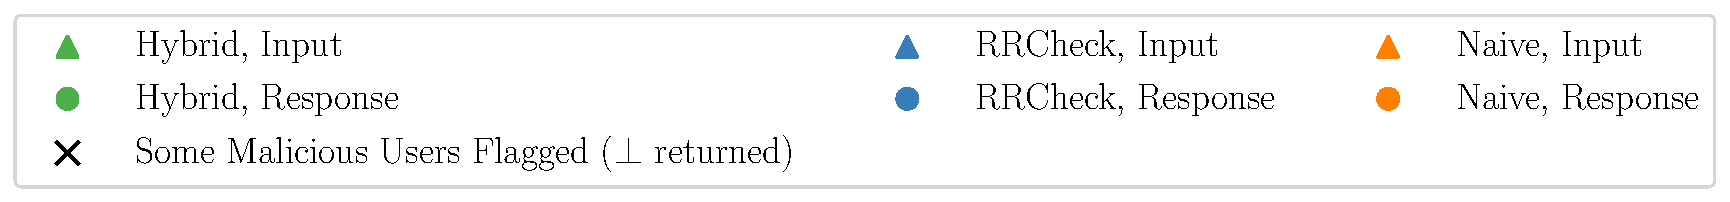
\includegraphics[width=0.8\linewidth]{Plots/legend.pdf}
        \end{subfigure}\\
 \begin{subfigure}[b]{\linewidth}
     
         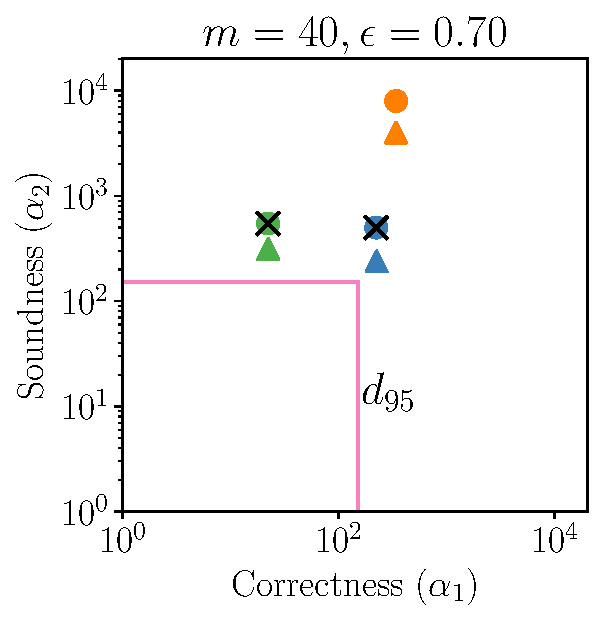
\includegraphics[width=0.23\linewidth]{Plots/fb_inf_40_0.7.pdf}
 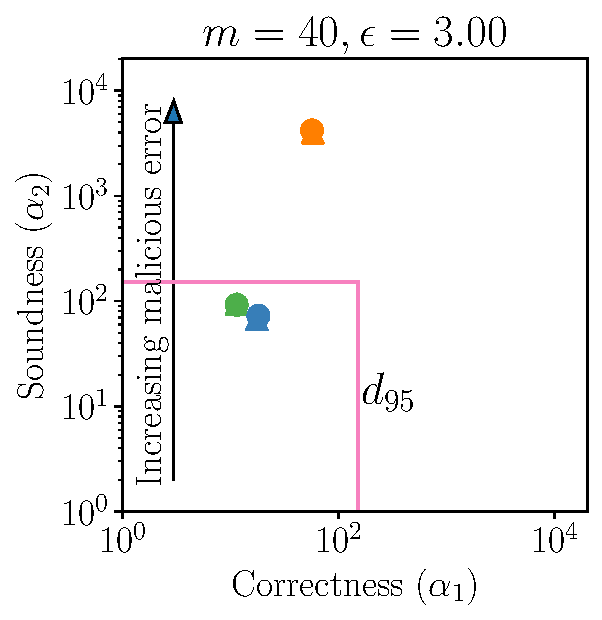
\includegraphics[width=0.23\linewidth]{Plots/fb_inf_40_3.0.pdf}   
  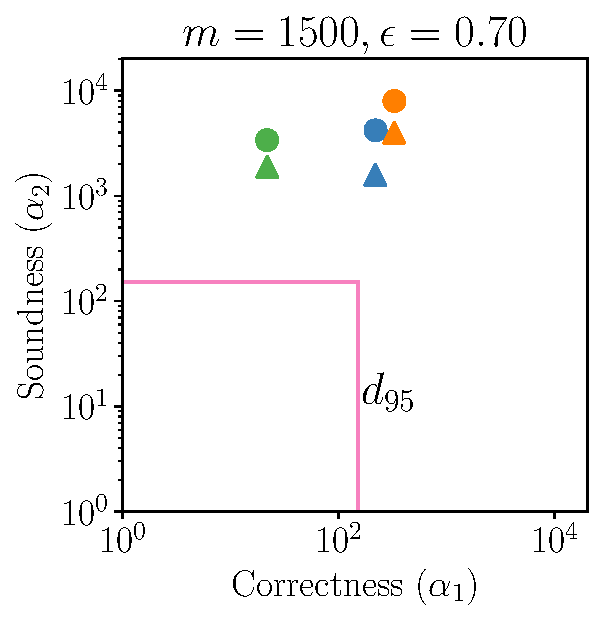
\includegraphics[width=0.23\linewidth]{Plots/fb_inf_1500_0.7.pdf} 
   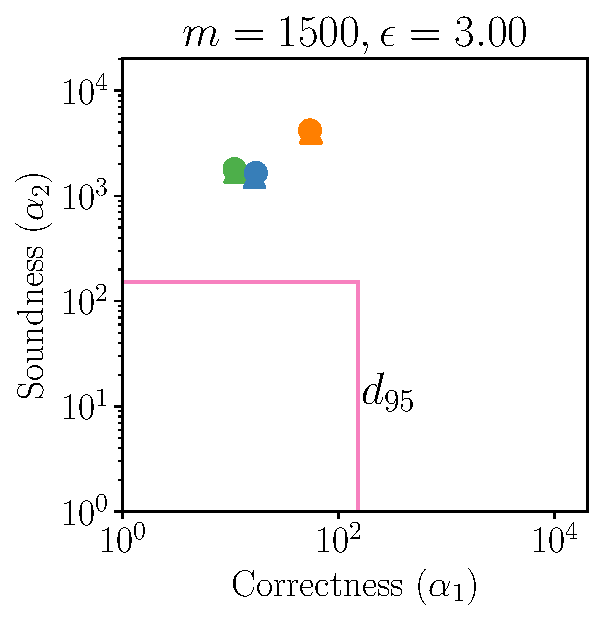
\includegraphics[width=0.23\linewidth]{Plots/fb_inf_1500_3.0.pdf} 
 \caption{\scalebox{0.8}{\textit{FB}: Degree Inflation Attack}}
        \label{fig:FB:infl}\end{subfigure}%%
    \\
    \begin{subfigure}[b]{\linewidth}
     
         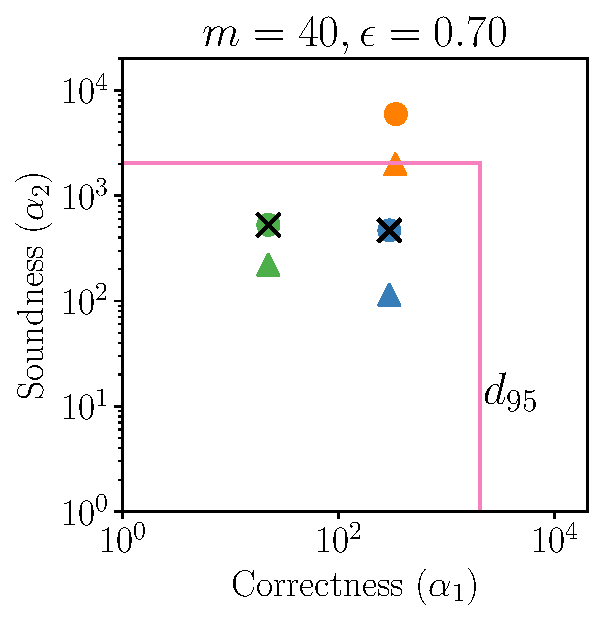
\includegraphics[width=0.23\linewidth]{Plots/gnm_inf_40_0.7.pdf}
 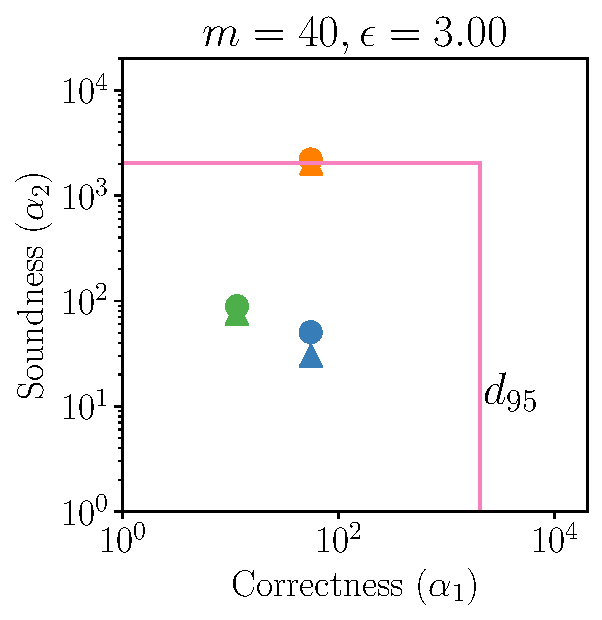
\includegraphics[width=0.23\linewidth]{Plots/gnm_inf_40_3.0.pdf}   
   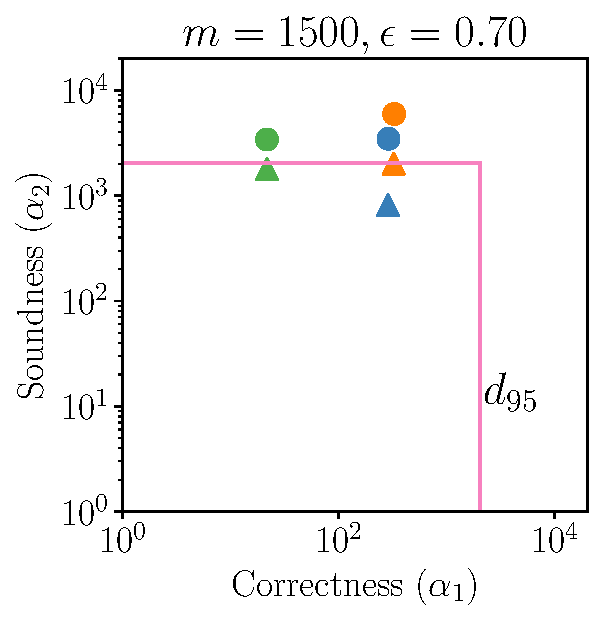
\includegraphics[width=0.23\linewidth]{Plots/gnm_inf_1500_0.7.pdf}
 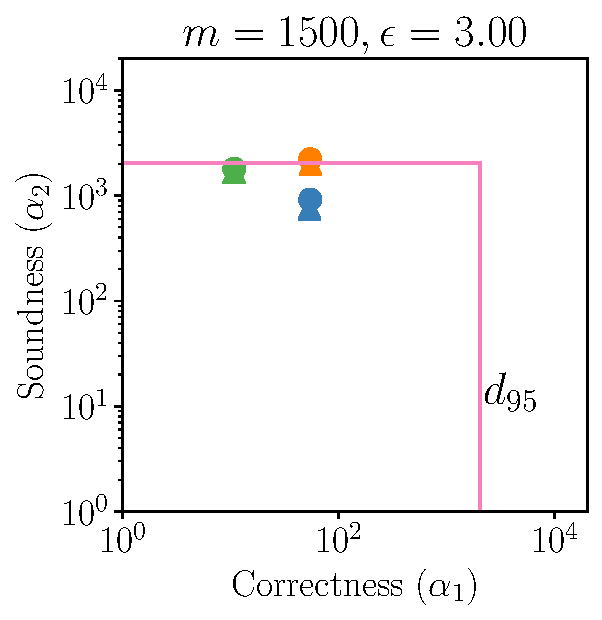
\includegraphics[width=0.23\linewidth]{Plots/gnm_inf_1500_3.0.pdf} 
\caption{\scalebox{0.8}{\textit{Syn}: Degree Inflation Attack}}
        \label{fig:syn:infl}\end{subfigure}%%
   
  \caption{Robustness Analysis for Degree Inflation Attack: We plot the empirical correctness (error of honest user) and soundness (error of malicious user). $d_{95}$ denotes the $95$-th percentile of the degree distribution.}
   \label{fig:analysis}%\vspace{-0.5cm}
\end{figure*}

\begin{figure*}[hbt!]
\begin{subfigure}[b]{\linewidth}

    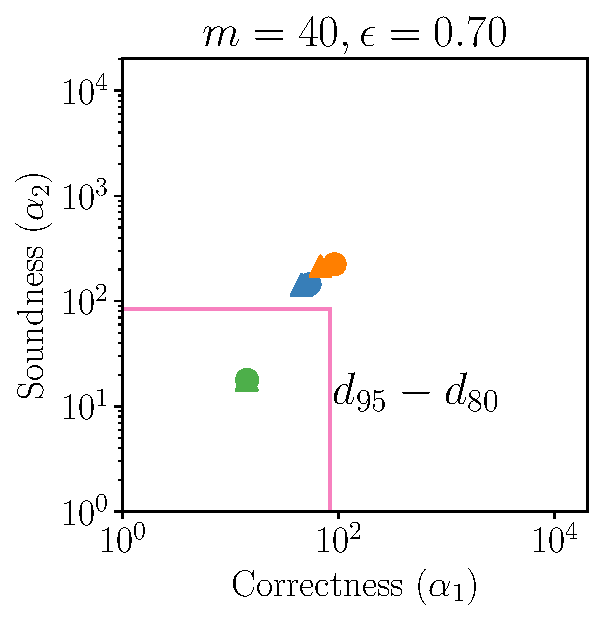
\includegraphics[width=0.23\linewidth]{Plots/fb_def_40_0.7.pdf}
 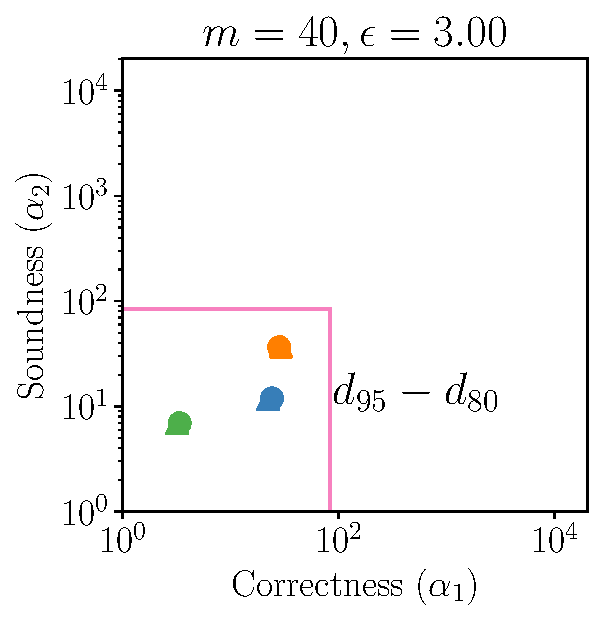
\includegraphics[width=0.23\linewidth]{Plots/fb_def_40_3.0.pdf}
    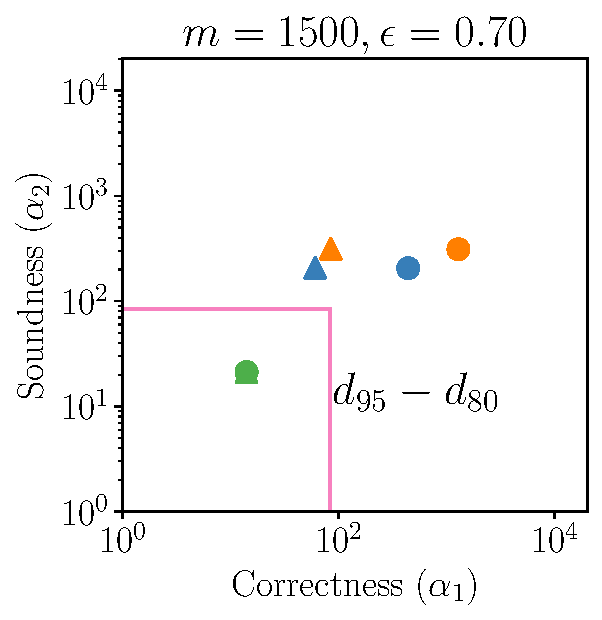
\includegraphics[width=0.23\linewidth]{Plots/fb_def_1500_0.7.pdf}
 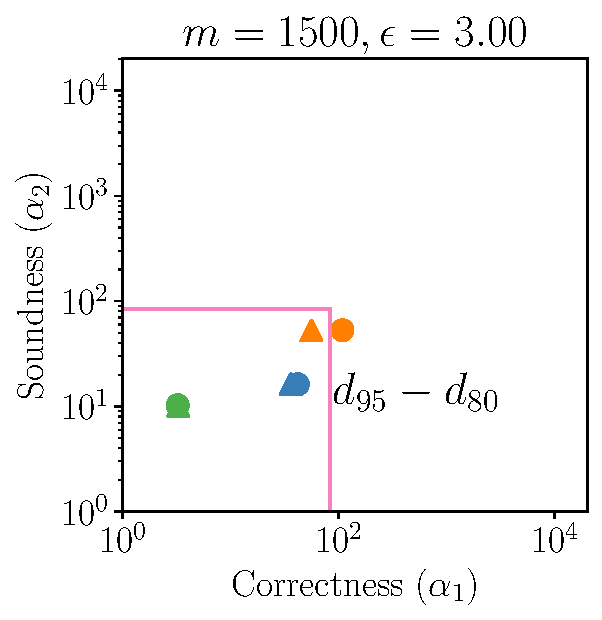
\includegraphics[width=0.23\linewidth]{Plots/fb_def_1500_3.0.pdf}
  \vspace{-0.2cm}  \caption{\scalebox{0.8}{\textit{FB}: Degree Deflation Attack}}
    \label{fig:FB:defl}
    \end{subfigure}\\
 \begin{subfigure}[b]{1\linewidth}
 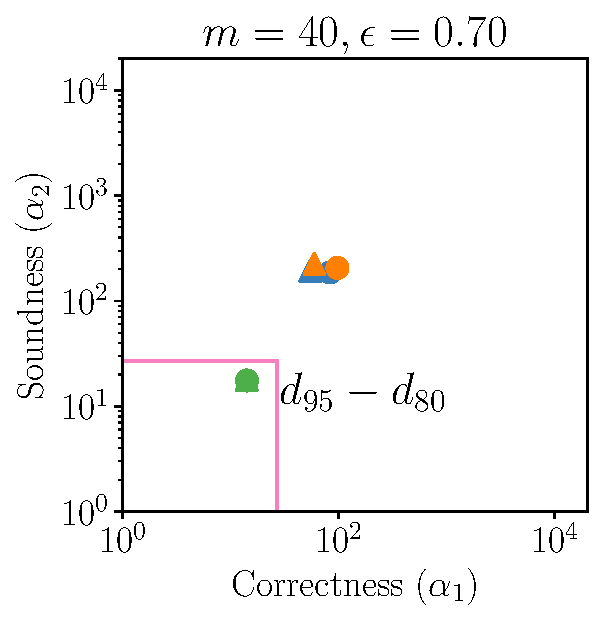
\includegraphics[width=0.23\linewidth]{Plots/gnm_def_40_0.7.pdf}
 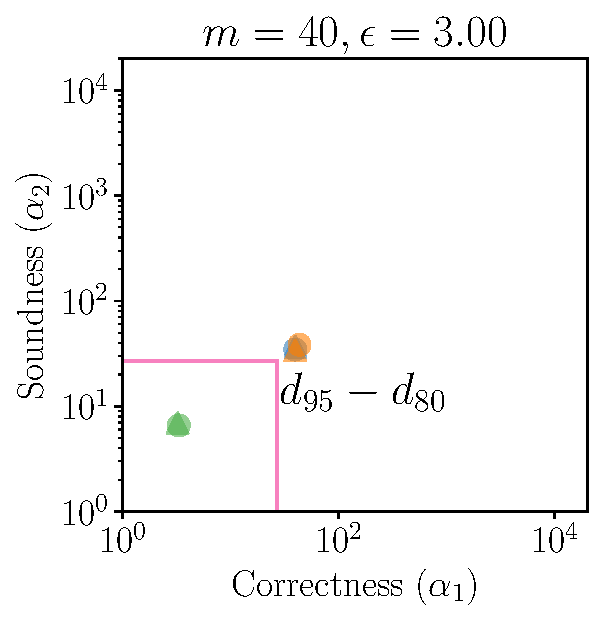
\includegraphics[width=0.23\linewidth]{Plots/gnm_def_40_3.0.pdf}
  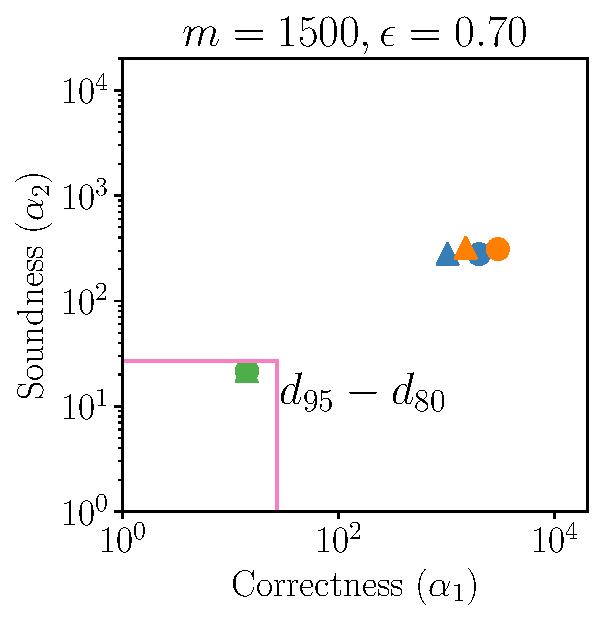
\includegraphics[width=0.23\linewidth]{Plots/gnm_def_1500_0.7.pdf}
 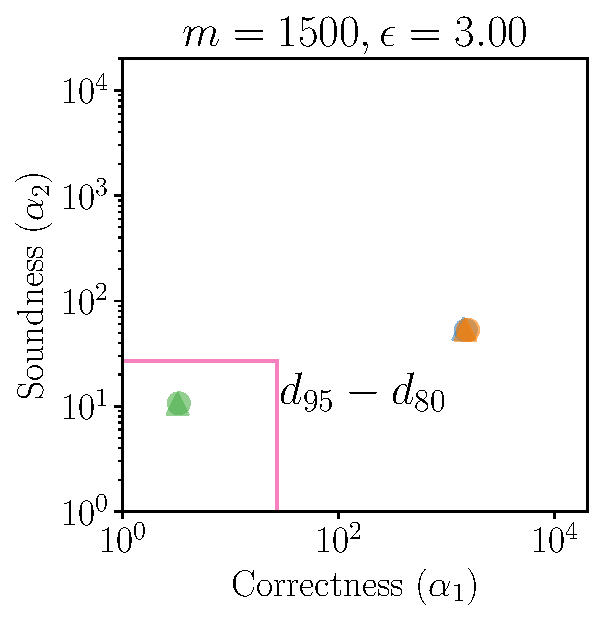
\includegraphics[width=0.23\linewidth]{Plots/gnm_def_1500_3.0.pdf}
  \vspace{-0.2cm}  \caption{\scalebox{0.8}{\textit{Syn}: Degree Deflation Attack}}
        \label{fig:Syn:defl}
        \end{subfigure}  \vspace{-0.5cm}  
\caption{Robustness Analysis for Degree Deflation Attack: We plot the empirical correctness (error of honest user) and soundness (error of malicious user). $d_{k}$ denotes the degree of the $k$ percentile node.}
\end{figure*}


\begin{figure}
  \begin{subfigure}[b]{0.49\linewidth}
    \centering 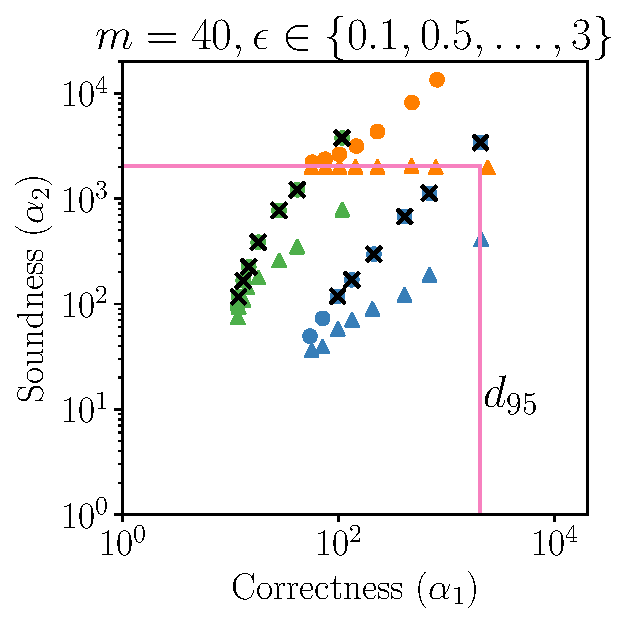
\includegraphics[width=1\linewidth]{Plots/gnm_inf_vary_40.pdf}  \vspace{-0.7cm}  
        \caption{\textit{Syn}: Degree Inflation Attack}
        \label{fig:Syn:privacy}\end{subfigure}
        \begin{subfigure}[b]{0.49\linewidth}
        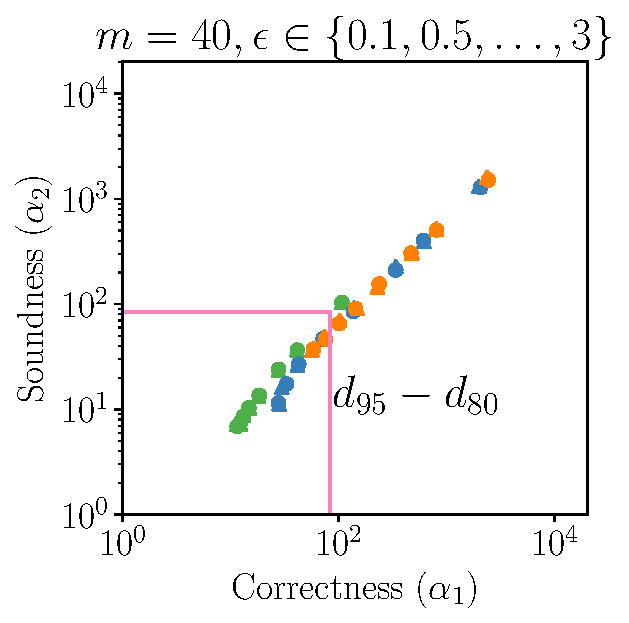
\includegraphics[width=\linewidth]{Plots/fb_def_vary_40.pdf}  \vspace{-0.7cm}  
        \caption{\textit{FB}: Degree Deflation Attack}
        \label{fig:FB:privacy}
        \end{subfigure}  \vspace{-0.3cm}  
\caption{Robustness analysis with varying $\epsilon$}
\end{figure}
\noindent \textbf{Protocols.} 
We evaluate our proposed \DegRRCheck{} and \DegHybrid{} protocols and use \DegRRNaive{} as a baseline protocol with poor robustness. %We ran each protocol on various graph datasets, with input and response poisoning attacks aimed at degree inflation and deflation, and with varying choices of parameters.
\vspace{-0.2cm}\\\\
\noindent\textbf{Attacks.} For each protocol, we evaluate two types of attacks -- degree inflation and degree deflation where the goal of the malicious users is to increase (resp. decrease) the degree estimate of a target malicious (resp. honest) user by as much as possible.
 We choose these attacks because firstly, they can meet the asymptotic theoretical error bounds.
%\footnote{Due to symmetry, attacks which target multiple users can be considered as a set of attacks with a single target. The only distinguishing feature is whether the targeted user is honest or malicious. Also due to symmetry, it is equivalent to consider either degree inflation or deflation attacks for one attacked target user, and the same for one target malicious user.}.
Secondly, these attacks are grounded in real-world motivations and represent practical threats (see Sec. \ref{sec:attacks}). For each attack type, we consider both input and response poisoning versions. In the following, let $\DO_t$ represent the target user. 
\vspace{-0.2cm}\\\\
\noindent\DegRRCheck{}. For the degree inflation attack, the non-target malicious users always report a $1$  for the malicious user $\DO_t$ (i.e. that they are connected to $\DO_t$) in the hopes of increasing $\DO_t$'s degree estimate.
Likewise, $\DO_t$ reports $1$s for all other malicious users. For the honest users, $\DO_t$ reports extra $1$s (for non-neighbors) in the hopes of further increasing their degree estimate. The exact mechanism depends on whether it is response poisoning or input poisoning and is detailed in App. \ref{app:attacks}.
\begin{comment}: For input poisoning, $\DO_t$ takes $q_1$ of their non-neighboring honest users and reports $1$. For response poisoning, $\DO_t$ simulates their true response by applying randomized response to his data, and then takes $q_1$ of the $0$s from that response and reports $1$s. During the trials, we used $q_1 = 15\%$, as at this threshold the chance of the $\DO_t$ being flagged as $\bottom$ became significant. For exact mechanisms for both input and response poisoning, see Appendix~\ref{app:attacks}.
\end{comment}

For degree deflation, we consider the worst-case scenario where $m$ of the neighbors of the honest user $\DO_t$ act maliciously. The malicious neighbors always report $0$ for their edges to $\DO_t$ (see App.~\ref{app:attacks}).
\vspace{-0.2cm}\\\\
\noindent\DegHybrid. %Recall that for this protocol, users report their edges via randomized response and a degree estimate $\tilde{d}_i^{lap}$ via the Laplace mechanism. 
For degree inflation, the non-target malicious users report their edges using the same strategy as in \DegRRCheck{}. For $\tilde{d}_i^{lap}$, they send their true degree estimates since their degrees are not the targets. Similarly, $\DO_t$ uses the same strategy as in $\DegRRCheck{}$ for reporting their edges. For $\tilde{d}_t^{lap}$, $\DO_t$  reports an inflated value based on the reported edges and the threshold $\tau$ (see  App. \ref{app:attacks}).

For degree deflation, we consider the worst-case scenario where $m$ of the neighbors of $\DO_t$ act maliciously. The malicious users behave as they did in \DegRRCheck{} and report their true degrees for $\tilde{d}_i^{lap}$, as these are not the targeted degrees.
\vspace{-0.2cm}\\\\
 \noindent\DegRRNaive. For degree inflation, we consider the worst-case scenario where the target malicious user $\DO_t$ is responsible reporting all their edges, and chooses to reports all $1$s. %For response poisoning, this is equivalent to Algorithm~\ref{alg:attack3}. For input poisoning, this is equivalent to running Algorithm~\ref{alg:attackinput} with all 1s as the poisoned input.

For degree deflation, we again consider the worst case scenario where the malicious users are responsible for reporting the edges to $\DO_t$, and they report $0$s.
\vspace{-0.2cm}\\\\
\noindent \textbf{Configuration.} %For each of the aforementioned graphs, we ran our three protocols against degree inflation and deflation attacks. 
 For degree inflation, we report the maximum error over all honest users (correctness, $\alpha_1$) and the error of the malicious target (soundness, $\alpha_2$). For degree deflation, we report the error of the honest target (correctness) and the maximum error over all the malicious users (soundness). We run each experiment $50$ times and report the mean.  We use $\delta=10^{-6}$ and $c = 0.9$ for \DegHybrid{}. Additional details are in App.~\ref{app:attacks}. %For each attack, we selected a random target user, and for degree inflation, we chose $m-1$ additional malicious users from the remaining nodes. For degree deflation, we selected a random target user and selected $m$ of that user's neighbors to be malicious. In degree inflation, we reported the error of the target's degree inflation (soundness) against the maximum error over all honest users (correctness). In degree deflation, we reported the maximum error of the malicious users' degrees (soundness) against the error of the target (correctness). %We performed both input and response versions of each attack type. We ran each attack version, including reselecting the target and malicious users, $50$ times and report the mean---if any user is flagged with $\bottom$, we simply report the mean over the smaller set. We use $\delta=10^{-8}$. .

\begin{comment}\begin{enumerate}\item Gap between theory and practice for degree vector \item Test other questions - \begin{itemize}\item degree histogram \item highest degree value \item highest degree node \end{itemize}\item Test adversary selection strategies \begin{itemize}\item adversaries belong to $k$-th percentile \item  target's degree \item malicious clients share an edge with the target vs do not share an edge \end{itemize}\end{enumerate}
\end{comment}
\vspace{-0.4cm}
\subsection{Results} \label{sec:exp-results}
%\arc{Report how many time the malicious user is caught for degree inflation}
 We consider two values of $m$ (number of malicious users): $m=40$ and $m=1500$. The former corresponds to $=1\%$ malicious users which represents a realistic threat model. We also consider $m=1500$ to showcase the efficacy of our protocols even with a large number of malicious users ($=37.5\%$).
\vspace{-0.2cm}\\\\\noindent\textit{Degree Inflation.} We report our results for degree inflation in Figs.~\ref{fig:FB:infl} and~\ref{fig:syn:infl}.  In terms of correctness, we observe that \DegHybrid{} performs the best --- this is expected since the error introduced by the Laplace mechanism of $\tilde{O}(\frac{1}{\epsilon})$ is the lowest. Both \DegRRCheck{} and \DegRRNaive{}  have higher honest error of $\tilde{O}(\frac{\sqrt{n}}{\epsilon})$ due to the underlying randomized response mechanisms. \DegRRCheck{} has better correctness than \DegRRNaive{}, particularly for \textit{FB} with low privacy ($\epsilon=3$). This is because the degree estimator for \DegRRNaive{} is based on the random variable $count^{1}$  (Sec. \ref{sec:protocol:naive}) which  has a variance $n\rho(1-\rho)$. However, the degree estimator for \DegRRCheck{} is based on the random variable $count^{11}$ (Sec. \ref{sec:protocol:check}). The variance of $count^{11}$ is a function of the graph degree distribution and is lower than that of $count^{1}$ for sparse graphs and high $\epsilon$. 
In terms of soundness, both our proposed protocols perform better than the baseline  -- \DegRRNaive{}  has $43\times$ and $60\times$ higher malicious error than \DegHybrid{} and \DegRRCheck, respectively, for \textit{FB} for $\epsilon=3, m=40$ for input poisoning. Note that \DegRRCheck{} performs slightly better than \DegHybrid. This is because, although both the protocols have the same asymptotic soundness guarantee, the constants are higher for \DegHybrid (see Sec. \ref{sec:hybrid}). %This is because the additional Laplace degree estimate gives an extra way for the malicious target to cheat, as described in the attacks section. However, as noted in Section~\ref{sec:hybrid:attack}, this difference is only up to constants, the asymptotic soundness guarantee of \DegRRCheck{} and \DegHybrid{} is the same. 
Finally, we observe that response poisoning is worse than input poisoning for all the protocols for soundness, which is to be expected and is consistent with the theory (response poisoning has an extra $O(\frac{m}{\epsilon}$) term). For instance, for \DegRRCheck{}, response poisoning is $4.2\times$ worse than input poisoning for \textit{Syn} with $m=1500,\epsilon=0.7$. As expected, the separation becomes less prominent with higher privacy and lower $m$, as it is harder to pull off strong attacks for these regimes.



\par Figs. \ref{fig:FB:infl} and \ref{fig:syn:infl} also mark the degree of $95^{th}$ percentile node ($d_{95}$) for the respective graphs. The way to interpret this is as follows.  If an error of a protocol falls outside the box, then any malicious user can inflate their degree estimate to be in the $>d_{95}$ percentile by staging a poisoning attack. Our protocols are better performant for the dense graph \textit{Syn} (attacks are prevented for both values of $\epsilon$). This is because of the $\tilde{O}(\frac{\sqrt{n}}{\epsilon})$ term in the soundness guarantee -- this term dominates the malicious error for sparse graphs. 

\par Finally, for both datasets for $m=40$ and $\epsilon = 0.7$, our protocols flag the malicious target user (returning $\bottom$) for $30\%-70\%$ of the trials.  We indicate this with an ``X'' in the figures. This indicates that our proposed protocols are able to detect malicious users, thereby disincentivizing malicious activity.
\vspace{-0.2cm}\\\\
\noindent\textbf{Degree Deflation.}
Figs. \ref{fig:FB:defl} and  \ref{fig:Syn:defl} show the results for the degree deflation attacks on  \textit{FB} and \textit{Syn}, respectively. We observe that \DegHybrid{} performs the best in terms of both correctness and soundness. For instance, it has $58\times$ and $20\times$ better correctness than \DegRRNaive{} and \DegRRCheck{}, respectively, for \textit{FB} and response poisoning with $\epsilon=0.7, m=1500$. $\DegRRCheck{}$ and $\DegRRNaive{}$ have similar correctness. This is because the correctness guarantees for both protocols are asymptotically the same. %The correctness of $\DegRRCheck{}$ is between that of $\DegHybrid{}$ and $\DegRRNaive{}$, and it is better than $\DegRRNaive{}$ by small factors between $1-2$. This is consistent with the theoretical results, as the correctness guarantees for both protocols are asymptotically the same.
The soundness error for these two protocols are from just the underlying randomized response mechanisms. We observe that \DegRRCheck{} has better soundness than  \DegRRNaive{} for \textit{FB} for $\epsilon=3$ because of a better degree estimator as described previously. Finally, we observe that the response poisoning is more damaging than input poisoning for \DegRRNaive{} and \DegRRCheck. For instance, response poisoning has $2\times$ worse correctness than input poisoning for \DegRRCheck{} for \textit{Syn} with $\epsilon=0.7,m=1500$. However, the two types of poisoning have a similar impact on the correctness of \DegHybrid{}, as the final degree estimate sent by the target user via the estimate from the Laplace mechanism is not poisoned.

We note that none of the degree deflation attacks resulted in the honest user being falsely flagged, demonstrating empirically  that our protocols do not have false positives.

We plot the measure $d_{95}-d_{80}$ in Figs. \ref{fig:FB:defl} and \ref{fig:Syn:defl} where $d_{k}$ denotes the degree of the $k$ percentile node. The way to interpret this is as follows. If an error falls outside the box, then malicious users can successfully deflate the degree of an honest target from $>95$ percentile to $<80$ percentile. Based on our results, we observe that \DegHybrid{} is mostly effective in protecting against this attack even with a large number of malicious users of $m=1500$. 
 %Additionally, 
%We make similar observations for the \textit{Syn} dataset (Fig. \ref{fig:Syn}) on all four attacks. The only distinction here is that, since \textit{Syn} is a dense graph, the relative error of \DegRRCheck$(\cdot)$ is significantly smaller than that for the sparse \textit{FB} graph. Hence, it might be acceptable to use \DegRRCheck$(\cdot)$ for dense graphs  especially for degree inflation type attacks.
\vspace{-0.2cm}\\\\
\noindent\textbf{The effect of $\epsilon$.} Figs. \ref{fig:FB:privacy} and \ref{fig:Syn:privacy} show the impact of the attacks with varying privacy parameter $\epsilon$. We observe that, increasing privacy (lower $\epsilon$) leads to more skew for all attacks on all three protocols. For instance, the response poisoning version of the degree deflation attack for \textit{FB}  is $74\times$ worse for $\epsilon=0.1$ than that for $\epsilon=3$ for \DegRRCheck{}. Additionally, we observe that malicious users get flagged only for input poisoning for larger $\epsilon$. This is because for small values of $\epsilon$, the thresholds are large due to more noise introduced by privacy which makes it harder to detect malicious users. 
\par Another interesting observation is that even a relatively small number of malicious parties ($m=1\%$) can stage significantly damaging poisoning attacks. This demonstrates the practical threat of such poisoning attacks. As expected, the impact of the poisoning attacks worsens with increasing $m$. Nevertheless, our results show that our proposed protocols are able to significantly reduce the impact of poisoning attacks even with a large number of malicious users ($m=37.5\%$).
%\arc{Input error higher than response \\Malicious error should be higher than honest error}
%This is a realistic assumption in many scenarios. Next, we considered a highly adversarial $1500$ adversaries. While many of the protocols do not perform well for this setting, this setting illustrates several important concepts for our protocol.

 %Our low value of $\epsilon$ is a strong privacy guarantee and serves to highlight the increased susceptibility of the protocols to attacks. Our higher value of $\epsilon$ is more in line with values typically used in practice.


\begin{comment}
\arc{Jotting down the main observations, their possible explanations and current anomalies (A) in the graph}
95th percentile gain not really --
Degree Inflation: FB
\begin{itemize}
\item No attack on honest users
    \item Response > Input for all settings, more prominent for low eps, high m - A: 5a.2 (sqrt{n}{eps} dominates) , 5a.2 Why is inout and response flipped for RRcheck? 5a. 4 -- sqrt{n}{eps} dominating despite high m?
    \item Why is the honest error increasing for RRcheck with high m - it should not be affected at all?
    \item Error for Naive does not increase because of our protocol - target had control over all edges 
    \item Hybrid has lowest honest error
    \item RRcheck has lower malicious error than Hybrid - order same, higher constants
    \item Honest error for Naive < for RRcheck - better estimator -A: M=40 and M=1500 contradictory
\end{itemize}

Degree Deflation: FB
\begin{itemize}
    \item Needs new deflation attack for RRNaive
    \item No malicious error
    \item A: Why is the difference between the response and input not prominent here even for low eps high m - acceptable for Hybrid?
    \item Honest/malicious error does not change with m for Hybrid
    \item A: Malicious error increases for RRcheck with m- why, honest error should increase more for RRcheck?
    
\end{itemize}

For Syn
\begin{itemize}
    \item A: what is the gain of RRcheck now is not clear
    \item A: M=1500 seems to be exactly the same as that of FB
\end{itemize}



In Figure~\ref{fig:my_label}, we plot the malicious error and honest error as a point for the \textit{FB} graph, for both degree inflation and degree deflation attacks, for two values of $m$ and $\epsilon$. Around each point, we also plotted an ellipse of radius $3$ times the sample standard deviations, indicating a $99\%$ chance that the true values lie within the ellipse. Note the ellipses are distorted due to the log axis. Often, the ellipse is smaller than the point and is not visible. We have the following findings.

First, it is often true that $\DegHybrid{}$ performs better than the other two protocols in terms of both honest and malicious error. The honest error is about $5$ to $10$ times better than the other two algorithms, and is never worse than about $40$ (for $\epsilon = 0.3$) and about $10$ (for $\epsilon = 3.1$). \arc{from Fig 5, the honest error of \DegHybrid~is never worse than the other two (as it should be) - why do you say "never worse than about $40$ (for $\epsilon = 0.3$) and about $10$ (for $\epsilon = 3.1$)" this then?} The other two algorithms have honest error of at least $600$ and $25$, respectively. For malicious error, a similar observation holds for the degree deflation attacks. However, for the degree inflation attacks, $\DegRRCheck{}$ outperforms $\DegHybrid$ by a factor of $2$ to $5$. For example, when $\epsilon = 3.1$ and $m=40$, the malicious error for response poisoning is $195$ for \DegHybrid{} and $35$ for \DegRRCheck{}. \arc{they are order optimal but \DegHybrid~has higher concrete constants due to the second check}

In comparing \DegRRCheck{} with \DegRRNaive{}, the former algorithm attains less honest error than the latter for $40$ adversaries by a factor of $1$ to $2$. \ji{Why is this true?}. However, for $1500$ adversaries, the \DegRRNaive{} attains less honest error by a factor of at least $5$. \DegRRCheck{} always attains less malicious error than \DegRRNaive{}, and for the degree inflation attacks, it obtains the best malicious error of $35, 82$ for response and input poisoning attacks for $\epsilon = 3.1$ on $40$ adversaries.

Second, in general the degree inflation attacks are effective at $\epsilon = 0.3$, where an adversary is able to add at least a few hundred to his degree. However, at $\epsilon = 3.1$, \DegRRCheck{} is resistant to poisoning, attaining honest error no more than $26$ and malicious error no more than $82$.
For degree deflation attacks, $\DegHybrid{}$ attains errors less than $40$ (resp. $10$) for $\epsilon = 0.3, 3.1$ at all numbers of adversaries.

Third, for degree inflation, input poisoning is generally a less effective than response poisoning, particularly at lower levels of privacy. For example, with $40$ adversaries, the malicious error inflicted on \DegHybrid{} is $1200, 2700$ for input and response poisoning, respectively. This ratio for the other mechanisms is even larger. However, for $\epsilon = 3.1$, the malicious errors of input and response poisoning converge, with less than a $5\%$ difference.
For degree deflation, there is no noticeable gap between input poisoning and response poisoning, except for \DegRRCheck{} when $\epsilon = 0.3$: there, input poisoning attains honest error of $1250$ while response poisoning attains honest error of $2530$.
\ji{Check why the input poisoning error is sometimes higher than the response poisoning error for the FB graph.}

\end{comment}

  \vspace{-0.4cm}  \subsection{Discussion}\label{sec:exp-discuss}
Here, we discuss our empirical results in the context of our three evaluation questions. First, we observe that the baseline protocol \DegRRNaive{}  performs worse than both our proposed protocols. \DegHybrid{} offers the best correctness guarantee and its soundness is at least comparable to that of \DegRRCheck{} for all the attacks. Concretely, \DegHybrid{} can improve the correctness  and soundness by up to $25\times$  and $58\times$, respectively, as compared to that for \DegRRNaive. Second, we observe that the response poisoning is stronger than input poisoning for all four attacks and all three protocols. Concretely, the response poisoning can be up to $4.2\times$ worse than input poisoning.
Finally, we see that the privacy exacerbates the impact of the poisoning attacks -- both correctness and soundness gets worse with lower values of $\epsilon$ for all attacks on all three protocols. Concretely, poisoning can worsen by up to $74\times$ for a drop in privacy from $\epsilon=3$ to $\epsilon=0.7$.
  \vspace{-0.2cm}  \section{Related Work}\label{chap4-sec:relatedwork}
%In this section, we discuss the relevant prior work.\\\\
\noindent\textbf{Data Poisoning for LDP.}   A recent line of work~\cite{Cheu21,Cao_USENIX21,Wu21,Li22} has explored the impact of poisoning attacks in the \ldp~setting. However, these works focused either on tabular data or key-value data. Additionally, prior work mostly focuses on the task of frequency estimation which is different from our problem of degree estimation. For the former, each user has some item from an input domain and the data aggregator wants to compute the histogram over all the users’ items. Whereas, we compute the degree vector $\langle \hat{d}_1, \ldots, \hat{d}_n\rangle$ -- each user directly reports their degree $d_i$ (a count or via an adjacency list). More specifically, Cao et al.~\cite{Cao_USENIX21} proposed attacks where  an adversary could increase the estimated frequencies for adversary-chosen target items or promote them to be identified as heavy hitters. Wu et al.~\cite{Wu21} extended the attacks  for key-value data where an adversary
aims to simultaneously promote the estimated frequencies and mean values for some adversary-chosen target keys. Both the works also presented some ad-hoc defenses against the proposed attacks. However, their efficacy is heavily dependent on instantiation specific factors such as the data distribution or the percentage of fake users. Cheu et al.~\cite{Cheu21} formally analyzed the poisoning attacks on categorical data and showed that local algorithms are highly vulnerable to adversarial manipulation -- when the privacy level is high or the input domain is large, an adversary who controls a small fraction of the users in the protocol can completely obscure the distribution of the users’ inputs. This is essentially an impossibility result for robust estimation of categorical data via non-interactive LDP protocols. Additionally, they showed that poisoning the noisy messages can be far more damaging than poisoning the data itself. A recent work~\cite{Li22} studies the impact of data poisoning for mean and variance estimation for tabular data. In the shuffle \DP~model, Cheu et al.\cite{Cheu22} have studied the impact of poisoning on histogram estimation. %It is important to note that in addition to the type of data, the problem setting considered in prior work on LDP is also fundamentally different from ours.  
In terms of general purpose defenses, prior work has explored strategies strategy based on cryptographically  verifying implementations of \ldp~randomizers~\cite{Kato21,Ambainis03,Moran06} -- this would restrict the class of poisoning attacks to input poisoning only. \\A slew of poisoning attacks~\cite{biggio2021poisoning,mei2015teaching,Fang2020LocalMP,bhagoji2019analyzing, chen2017targeted,bagdasaryan2018backdoor,Xie2020DBADB} on machine learning (ML) models have been proposed in the federated learning setting~\cite{kairouz2019advances}. %The attacks could be either untargeted where the attack goal is to reduce the overall model accuracy~\cite{}, or targeted where backdoors are injected for certain target classes~\cite{}. 
A recent line of work \cite{roychowdhury2021eiffel, burkhalter2021rofl} explores defense strategies based on zero-knowledge proofs that aim to detect the poisoned inputs. Note that the aforementioned poisoning attacks on ML models are fundamentally different from the ones in our setting. For ML, the users send parameter gradient updates (multi-dimensional real-valued vector) and the attack objective is to misclassify data. On the other hand, our input here is a binary vector/single integral value with an underlying graphical structure and the attack objective is to perturb the degree estimates. Hence, none of the techniques from this literature are directly applicable to our setting.
  \vspace{-0.2cm}  \\\\
\noindent\textbf{LDP on Graphs.} DP on graphs has been widely studied, with most prior work being in the centralized model \cite{blocki2012johnson,Graph2,Graph3,Graph4,Graph5,Graph6,Graph7,Graph8,Song_arXiv18,Graph10}. 
In the local model, there exists work exploring the release of data about graphs in various settings ~\cite{LDPGraph1,LDPGraph2,LDPGraph3,LDPGraph4,LDPGraph5,LDPGraph6}. Recent work exploring private subgraph counting~\cite{imola2021locally,imola_communication-efficient_2022} is the most relevant to our setting, as the degree information is the count of an edge, the simplest subgraph. However, no previous work explores poisoning \ldp~protocols in the graph setting.

  \vspace{-0.2cm}  \section{Conclusion}\label{chap4-sec:conclusion}

In this paper, we have investigated the impact of poisoning attacks on degree estimation for graphs under \ldp. We have presented a formal framework for analyzing the robustness of a protocol against poisoning. Our framework can quantify the impact of a poisoning attack on both honest and malicious users. 
Additionally, we have proposed novel robust degree estimation protocols under \ldp~by leveraging the natural data redundancy in graphs, that can significantly reduce the impact of poisoning attacks.
%\noindent \textbf{Acknowledgements.} This material is partially based upon work supported by the National Science Foundation under Grant \# 2127309 to the Computing Research Association for the CIFellows Project.
%Kamalika Chaudhuri and Jacob Imola would like to thank ONR under N00014-20-1-2334 and NSF under CNS 180429 for research support.


%-------------------------------------------------------------------------------

%\bibliographystyle{ACM-Reference-Format}
\bibliographystyle{plain}
\bibliography{references}
\appendix
\graphicspath{{./chapters/chapter4/}}
\chapter{ }

\section{Background Cntd.}\label{app:background}


\setlength{\textfloatsep}{2pt}
%\begin{algorithm}
%  \caption{$\rr_\rho: \{0,1\}^n\mapsto\{0,1\}^n$ }\label{alg:rr}
%  \begin{algorithmic}[1]
%  \Statex \textbf{Parameters:} $\epsilon$ - Privacy parameter;
%  
%  \Statex\textbf{Input:} $l \in \{0,1\}^n$ - True adjacency list;
%  \Statex \textbf{Output:} $q \in \{0,1\}^n$ - Reported (noisy) adjacency list;
%  \vspace{0.2cm}
%  \State $\rho=\frac{1}{1+e^{\epsilon}}$
%  \For{$i \in [n]$}
%  \State $q[i]=\rr_\rho(l[i])$
%  \EndFor
%  \Return $q$
%  \end{algorithmic}
%\end{algorithm}
\begin{algorithm}
  \KwData{$l \in \{0,1\}^n$ - True adjacency list}
  \KwResult{$q \in \{0,1\}^n$ - Reported (noisy) adjacency list}
  $\rho=\frac{1}{1+e^{\epsilon}}$\;
  \For{$i \in [n]$}{
  	$q[i]=\rr_\rho(l[i])$\;
	}
  \KwRet $q$
  \caption{$\rr_\rho: \{0,1\}^n\mapsto\{0,1\}^n$ }\label{alg:rr}
\end{algorithm}

\section{Proofs}\label{app:proofs}
First, we introduce notation and preliminary results used in our proofs.
\subsection{Notation} In this section, for a graph $G$ with vertices $[n]$, we let $d_i(S)$ for $S \subseteq [n]$ denote the number of neighbors of node $i$ in the set $S$.
We will often abuse notation for a set $\calS$ of users by also letting $\calS$ be the indices of the users in the set. Thus, we may let $i \in \calS$ be the index of some user in $\calS$.
Finally, we sometimes refer to user $\DO_i$ simply as user $i$.

\subsection{Preliminary Results}
We will heavily make use of the following concentration result:

\begin{lemma}\label{lem:bern-concentration}
    Let $X_1, \ldots, X_n$ denote independent random variables such that $X_i \sim \bern(p_i)$. Let $v = \sum_{i=1}^n p_i(1-p_i)$, and $X = \sum_{i=1}^n X_i$. Then,
    \begin{align*}
        \Pr[|X - \E[X]| \geq \max\{1.5 \ln \frac{2}{\delta}, \sqrt{2v\ln \frac{2}{\delta}}\}] &\leq \delta.
    \end{align*}
\end{lemma}
\begin{proof}
    Center the random variables so that $Z_i = X_i - p_i$; the variance $v$ does not change. We know by Bernstein's inequality that for all $t \geq 0$,
    \[
        \Pr[Z \geq t] \leq \exp\left(\frac{-t^2}{2(v + t / 3)}\right) \leq \exp\left(- \max \left\{ \frac{t^2}{2v}, \frac{3t}{2}\right\}\right).
    \]
    Thus, if $t \geq \max\{\frac{3}{2} \ln \frac{2}{\delta}, \sqrt{2 v \ln \frac{2}{\delta}}\}$, then $\Pr[Z \geq t] \leq \frac{\delta}{2}$. Applying the argument to $-Z$, we obtain the two-sized bound.
    
\end{proof}

Next, we observe the following facts about randomized response.
\begin{fact}\label{fact:rr-exp}
If user $i \in \calH$, then $\E[q_i[j]] = \rho + (1-2\rho) d_i(j)$.
\end{fact}

\begin{fact}\label{fact:2rr-exp}
If users $i,j \in \calH$, then $\E[q_i[j]q_j[i]] = \rho^2 + (1-2\rho) d_i(j)$.
\end{fact}
\subsection{Proof of Theorem \ref{thm:response:laplace}}\label{app:thm:response:laplace}
Recall that in the Laplace mechanism, a user's degree estimate $\hat{d}_i$ is simply $d_i + L_i$, where $L_i \sim Lap(\frac{1}{\epsilon})$ is a Laplace random variable generated by the user.\\\\\noindent
\textbf{Correctness.} The correctness guarantee follows from the concentration of Laplace distribution: Each Laplace random variable $L_i$ satisfies $|\Pr[|L_i| \geq t] \leq e^{-t\epsilon}$. Setting $t = \frac{1}{\epsilon}\ln \frac{n}{\delta}$ and applying the union bound, each of the $n$ Laplace variables will satisfy $|L_i| \leq \frac{1}{\epsilon}\ln \frac{\delta}{n}$ with probability $1-\delta$, and if this holds, then $|d_i - \hat{d}_i| \leq \frac{1}{\epsilon}\ln \frac{\delta}{n}$ for honest users.
\\
\noindent\textbf{Tight Soundness.} Consider the empty graph. A malicious user $\DO_i$ may report $n-1$, the maximum possible degree, and thus $\hat{d}_i = n-1$ while $d_i = 0$.

\subsection{Proof of Theorem~\ref{thm:response:naive}}\label{app:thm:response:naive}
\noindent \textbf{Correctness.}

As defined in \DegRRNaive{}, the estimator $count_i^1$ is given by 
\begin{gather}count^1_i=(\sum_{j < i} q_j[i] + \sum_{i < j} q_i[j])\end{gather}
We may alternatively split the above sum into honest bits and malicious bits as $count^1_i = hon_i + mal_i$. Here, 
\begin{gather*}
hon_i = \sum_{j < i, j \in \calH} q_j[i] + \sum_{i < j} q_i[j] \\
mal_i = \sum_{j < i, j \in \calM} q_j[i].
\end{gather*}
Since all bits in the sum $hon_i$ are honest, by Fact~\ref{fact:rr-exp} we have $\E[hon_i] = \rho|\calH_i| + (1-2\rho) d_i(\calH_i)$, where $\calH_i = \calH \cup \{1, 2, \ldots, i-1\}$. 

Furthermore, $0 \leq mal_i \leq |\calM_i|$, where $\calM_i = [n] \setminus \calH_i$. This implies $|mal_i - E_{mal,i}| \leq |\calM_i|$, where $E_{mal,i} = \rho|\calM_i| + (1-2\rho) d_i(\calM_i)$.
By Lemma~\ref{lem:bern-concentration} and a union bound, with probability $1-\delta$, we have for all $i \in \calH_i$ that
\begin{gather*}
\left|hon_i - \E[hon_i] + mal_i - E_{mal,i} \right| \leq  \sqrt{2\rho n \ln \frac{2n}{\delta}} + |\calM_i| \\ 
\implies \left|count_i^1 - \rho n - (1-2\rho)d_i \right| \leq  \sqrt{2\rho n \ln \frac{2n}{\delta}} + m \\ 
\implies |\hat{d}_i - d_i | \leq \frac{1}{1-2\rho} \sqrt{2\rho n \ln \frac{2n}{\delta}} + \frac{m}{1-2\rho}.
\end{gather*}

\noindent\textbf{Tight Soundness.} Consider the empty graph, and suppose that user $n$ is malicious. Since this user reports all his edges, he may report $q_i[j] = 1$ for all $j < 1$. Thus, $\hat{d}_n \geq n-1$, but $d_n = 0$, showing $n-1$-tight soundness.

\subsection{Proof of Theorem~\ref{thm:response:check}} \label{app:b3a3}
Recall the key quantities defined in \DegRRCheck{} (Algorithm~\ref{alg:degrrcheck}):
\begin{gather}
      count_i^{11} = \sum_{j \in [n] \setminus i} q_{i}[j] q_{j}[i] \\
      count_i^{01} = \sum_{j \in [n] \setminus i} (1-q_{i}[j])q_{j}[i].
\end{gather}
We now prove correctness.

\noindent \textbf{Correctness.} 
It will be helpful to split $count_i^{11} = hon_i^{11} + mal_i^{11}$, where $hon_i^{11} = \sum_{j \in \calH \setminus i} q_{i}[j] q_{j}[i]$ and $mal_i^{11} = \sum_{j \in \calM \setminus i} q_{ij} q_{ji}$. We define $hon_i^{01}$ and $mal_i^{01}$ similarly such that they satisfy $count_i^{01} = hon_i^{01} + mal_i^{01}$. We break the proof into two claims: showing that honest users receive an accurate estimate and that they are not disqualified.

\begin{claim}\label{claim:honest-response-concentration-1} We have
\[
    \Pr[\forall \DO_i \in \calH.~|\hat{d}_i - d_i| \geq \tfrac{m + 2 \sqrt{\rho n \ln \frac{4n}{\delta}}}{1-2\rho}] \leq \frac{\delta}{2}.
\]
\end{claim}
\begin{proof} 
Let $\DO_i \in \calH$. Then, $hon_i^{11}$ is a sum of $h-1$ Bernoulli random variables with $p = \rho^2$ or $(1-\rho)^2$. By Fact~\ref{fact:2rr-exp}, we have
\begin{align*}
    \E[hon_i^{11}] &= \rho^2 (h-1) + (1-2\rho) d_i(\calH)
\end{align*}
Now, $v$ defined in Lemma~\ref{lem:bern-concentration} satisfies $(h-1) \rho^2 \leq v \leq (h-1)(1-(1-\rho)^2) \leq 2(h-1)\rho$. Applying the Lemma and a union bound, we have with probability at least $1-\frac{\delta}{2}$ that for all $i \in \calH$,
\begin{equation}\label{eq:hon-player-bits}
    |hon_i^{11} - \E[hon_i^{11}]| \leq 2\sqrt{(h-1)\rho \ln \tfrac{4n}{\delta}}.
\end{equation}

On the other hand, we have that $0 \leq mal_i^{11} \leq m$, so if we let $E_{mal,i}^{11} = \rho^2 m + (1-2\rho) d_i(\calM)$ (defined for convenience later), then $|mal_i^{11} - E_{mal,i}^{11}| \leq m$.

Applying the triangle inequality, the following holds over all $i \in \calH$:
\begin{align*}
&|hon_i^{11} - \E[hon_i^{11}] + mal_i^{11} - E_{mal,i}^{11}|
\leq m + 2\sqrt{ \rho n \ln \tfrac{4n}{\delta}} \\
& \implies |count_i^{11} - \rho^2 (n-1) - (1-2\rho) d_i| \leq m + 2\sqrt{ \rho n \ln \tfrac{4n}{\delta}} \\
& \implies |\hat{d}_i - d_i| \leq \frac{m + 2\sqrt{ \rho n \ln \tfrac{4n}{\delta}}}{1-2\rho}
\end{align*}
This proves the claim.
\end{proof}
Next, we show that honest users are not likely to be disqualified.
\begin{claim}\label{claim:honest-response-concentration-2} We have
\[
    \Pr[\forall \DO_i \in \calH.~|count_i^{01} - \rho(1-\rho)(n-1)| \geq \tau] \leq \frac{\delta}{2},
\]
\end{claim}
where $\tau = m + \sqrt{2 \rho n \ln \frac{4 n}{\delta}}$

\begin{proof}
Let $\DO_i$ be honest. Then, the quantity $hon_i^{01}$ consists of $h-1$ Bernoulli random variables drawn from $\rho(1-\rho)$. We have
\[
    \E[hon_i^{01}] = \rho(1-\rho)(h-1).
\]
 As defined in Lemma~\ref{lem:bern-concentration}, $v$ satisfies $\frac{1}{2}(h-1)\rho \leq P \leq (h-1)\rho$.
Applying the Lemma and a union bound, we have with probability $1-\frac{\delta}{2}$ that for all $i \in \calH$, 
\begin{equation}\label{eq:hon-player-bits-2}
    |hon_i^{01} - \E[hon_i^{01}]| \leq \sqrt{2\rho (h-1) \ln \tfrac{4n}{\delta}}
\end{equation}
Noticing that $|mal_i^{01} - m \rho(1-\rho)| \leq m$, we have by the triangle inequality that
\[
    |count_i^{01} - \rho(1-\rho)(n-1)| \geq m + \sqrt{2\rho n \ln \tfrac{4n}{\delta}}.
\]
This concludes the proof.
\end{proof}
Putting it together,
$\left( m (\frac{e^\epsilon+1}{e^{\epsilon}-1}) + \sqrt{n}\frac{2 \sqrt{(e^\epsilon+1)\ln \frac{4n}{\delta}}}{e^\epsilon-1}, \delta\right)$-correctness follows.

\noindent \textbf{Soundness.} 

When player $i$ is a malicious player, we can still prove a tight bound on $count_{i}^{11} + count_{i}^{01}$, and this combined with the check in \DegRRNaive{} means that his degree estimate will be accurate.

\begin{claim}\label{claim:mal-response-concentration}
We have
\begin{multline*}
    \Pr[\forall i \in \calM.~|count_i^{11} + count_i^{01} \\ 
			-(1-2\rho)d_i - \rho(n-1)| \leq \tau ] \geq 1-\delta,
\end{multline*}
where $\tau = m + \sqrt{2 \rho n \ln \frac{4 n}{\delta}}$.
\end{claim}
\begin{proof}
Observe that $count_i^{11} + count_i^{01} = \sum_{j=1, j\neq i}^n q_{j}[i]$. Let $hon_i^{1}$ denote the sum of the $q_{j}[i]$ where $j$ is honest, and $mal_i^{1}$ denote the sum of the malicious players. By Fact~\ref{fact:rr-exp}, we have $\E[hon_i^1] = d_i(\calH) (1-2\rho) + h \rho$. Applying a union bound over Lemma~\ref{lem:bern-concentration}, for all $i \in \calM$, we have with probability at most $\delta$ that
\begin{equation}\label{eq:good-event-3}
    |hon_i^1 - \E[hon_i^1]| \geq \sqrt{2\rho n \ln \tfrac{2m}{\delta}}
\end{equation}
Because $|mal_i^1 - (1-2\rho)d_i(\calM) - \rho (m-1)| \leq m$, the claim follows from the triangle inequality.
\end{proof}

To conclude the proof, consider any malicious user $i \in \calM$ is not disqualified ($\hat{d}_i \neq \bottom$),
as if he is then the soundness event trivially happens. Thus, it must be true that $|count_i^{01} - (n-1)\rho(1-\rho)| \leq \tau$. However, given this and the event in Claim~\ref{claim:mal-response-concentration} holds, it follows by the triangle inequality that
\begin{align*}
    |count_i^{11}-(1-2\rho)d_i - \rho^2(n-1)| &\leq 2 \tau \\
    |\hat{d}_i - d_i| &\leq \frac{2 \tau }{1-2\rho}
\end{align*}
This establishes $\left( 2m (\frac{e^\epsilon+1}{e^{\epsilon}-1}) + 4\sqrt{n}\frac{ \sqrt{(e^\epsilon+1)\ln \frac{4n}{\delta}}}{e^\epsilon-1}, \delta\right)$-soundness.

\subsection{Proof of Theorem \ref{thm:no privacy}}\label{app:thm:no privacy}
\textbf{Correctness.}
Let honest $\DO_i$ share an edge with all malicious users in $\calM$. Now, all the malicious users can lie and report $0$ for $\DO_i$, i.e., set $q_j[i]=0 \forall j \in \calM$. This deflates $\DO_i$'s degree by $m$.
\\
\noindent \textbf{Soundness.} Let malicious $\DO_i$ share an edge with all users in the graph. Consider the attack where $\DO_i$ and $\DO_j, j \in \calM \setminus i$ report $0$ for their edges, and additionally $\DO_i$ reports $0$ for $\min\{m-1, n-m\}$ additional honest users. In this way, $\DO_i$ can deflate its degree estimate by $\min(2m-1,n)$.

\subsection{Proof of Theorem~\ref{thm:rrlapchecka3}}
\textbf{Correctness.}\label{app:thm:rrlapchecka3}
By Claim~\ref{claim:honest-response-concentration-2}, the first check in \DegHybrid{} will not set $\hat{d}_i = \bottom$ for any honest user with probability at least $1-\frac{\delta}{4}$. 
The variables $\hat{d}_i^{rr}$ in $\DegHybrid$ behave identically to $\hat{d}_i$ in \DegRRCheck{}. By Claim~\ref{claim:honest-response-concentration-1} 
we have for all users, $|\hat{d}_i^{rr} - d_i| \leq \frac{m + 2 \sqrt{\rho n \ln \frac{8n}{\delta}}}{1-2\rho}$,
with probability at least $1-\frac{\delta}{4}$. 

By concentration of Laplace random variables, we have for all $i \in \calH$ that $|\hat{d}_i^{lap} - d_i| \leq \frac{1}{\epsilon} \ln \frac{2n}{\delta}$ with probability at least $1-\frac{\delta}{2}$, 
and by the triangle inequality we have $|\hat{d}_i^{lap} - \hat{d}_i^{rr}| \leq \frac{m + 2 \sqrt{\rho n \ln \frac{8n}{\delta}}}{1-2\rho} + \frac{1}{\epsilon}\ln \frac{2n}{\delta}$. Thus, the second check will not set $\hat{d}_i = \bottom$ assuming these events hold, and the estimator $\hat{d}_i$ satisfies the correctness bound of $\hat{d}_i^{lap}$.

\textbf{Soundness.}
Following the same argument we saw in the soundness proof of Theorem~\ref{thm:response:check}, we can have that, with probability at least $1-\frac{\delta}{2}$, for all malicious users $i \in \calM$, we have $|\tilde{d}_i^{rr} - d_i| \leq \frac{2\tau}{1-2\rho}$. Suppose that $\hat{d}_i$ is not set to be $\bottom$. This implies that $|\tilde{d}_i^{rr} - \tilde{d}_i^{lap}| \leq \frac{2\tau}{1-2\rho} + \frac{1}{\epsilon}\log \frac{2n}{\delta}$.  By the triangle inequality, this implies
\[
    |\tilde{d}_i^{rr} - d_i| \leq \frac{4\tau}{1-2\rho} + \frac{1}{\epsilon} \log \frac{2n}{\delta}.
\]
This establishes $(\frac{4\tau}{1-2\rho} + \frac{1}{\epsilon} \log \frac{2n}{\delta}, \delta)$-soundness.

\subsection{Proof of Theorem~\ref{thm:input:laplace}}\label{app:thm:input:laplace}
\textbf{Correctness.} The correctness guarantee follows in the same way as Theorem~\ref{thm:response:laplace}.
\\
\noindent \textbf{Soundness.} Consider a malicious user $\DO_i$, and let $m_i$ be the malicious degree estimate sent by $\DO_i$, with $0 \leq m_i \leq n-1$. The estimator is given by $\hd_i = m_i+\eta, \eta \sim Lap(\frac{1}{\epsilon})$. 
Thus, $\Pr[|d_i - m_i - \eta| \geq n-1] \leq \Pr[\eta > 0] \leq \frac{1}{2}$.


\subsection{Proof of Theorem~\ref{thm:b2a2_easy}} \label{app:thm:b2a2_easy}
\noindent \textbf{Correctness.}
We follow the correctness proof of Theorem~\ref{thm:response:naive}, with the following change. Observe that $mal_i$ consists of $|\calM_i|$ Bernoulli random variables of mean either $\rho$ or $1-\rho$. Thus, with probability $1-\frac{\delta}{2}$, we have $|mal_i - \E[mal_i]| \leq \sqrt{2m\ln \frac{4m}{\delta}}$ for all $i \in \calM$. 

Thus, we can show $|mal_i - E_{mal,i}| \leq (1-2\rho) |\calM_i|$, where $E_{mal,i} = \rho |\calM_i| + (1-2\rho)d_i(M_i)$.
Finishing the proof, we can show 
\[
|\hat{d}_i - d_i | \leq \frac{1}{1-2\rho} (\sqrt{2\rho n \ln \tfrac{4n}{\delta}} + \sqrt{2m \ln \tfrac{4m}{\delta}}) + m.
\]
\noindent \textbf{Soundness.}

In order for $|d_i - \hat{d}_i| = n-1$, it is necessary for $|count_i^{1} - \rho(n-1) - (1-2\rho)d_i| \geq (1-2\rho)(n-1)$. We have $count_i^1$ is a sum of $n-1$ Bernoulli random variables of mean either $\rho$ or $1-\rho$, so it can be written as $\mu + Z_i$, where $Z_i$ is approximately a normal random variable of mean $0$. Observe that, since $\mu$ and $\rho(n-1) + (1-2\rho)d_i$ are in the interval $[\rho (n-1), (1-\rho)(n-1)]$, it is impossible for the difference $\mu - \rho(n-1) + (1-2\rho)d_i$ to exceed $(1-2\rho)(n-1)$ unless $Z_i$ has the correct sign, which happens with probability at most $\frac{1}{2}$. This establishes $(n-1, \frac{1}{2})$-soundness.
\subsection{Proof of Theorem~\ref{thm:input:check}}\label{app:b3a2}

\textbf{Correctness.}
Our proof follows that of Theorem~\ref{thm:response:check}. We are able to prove stronger versions of the claims.

\begin{claim}\label{claim:honest-input-concentration-1}
We have
\[
    \Pr[\forall i \in \calH.~|\hat{d}_i - d_i| \geq m+\frac{\sqrt{8\max\{\rho n, m\} \ln \frac{8n}{\delta}}}{1-2\rho}] \leq \frac{\delta}{2}.
\]
\end{claim}

\begin{proof}
We can control $hon_i^{11}$ in exactly the same way as in Claim~\ref{claim:honest-response-concentration-1}, so~\eqref{eq:hon-player-bits} holds with probability $1-\frac{\delta}{4}$, for all $i \in \calH$.
On the other hand, we know that $mal_i^{11}$ is now a sum of $d_i(\calM)$ Bernoulli random variables with bias either $(1-\rho)^2$ or $(1-\rho)\rho$, plus a sum of $m - d_i(\calM)$ Bernoulli random variables with bias either $\rho(1-\rho)$ or $\rho^2$. Thus, 
\begin{multline*}
	\rho(1-2\rho)d_i(\calM) + \rho^2 m \leq \E[mal_i^{11}] \\
	\leq (1-\rho)(1-2\rho)d_i(\calM) + \rho(1-\rho) m.
\end{multline*}
From this, we can show $|\E[mal_i^{11}] - E_{mal,i}^{11}| \leq (1-2\rho)m$, where $E_{mal,i}^{11} = \rho^2 m + (1-2\rho) d_i(\calM)$.
 Applying Hoeffding's inequality, we conclude that with probability at least $1 - \frac{\delta}{4}$, for all $i \in \calH$,
\[
    |mal_i^{11} - \E[mal_i^{11}]| \geq \sqrt{2m \ln \tfrac{8n}{\delta}}
\]
Thus, $|mal_i^{11} - E_{mal,i}^{11}| \leq (1-2\rho)m + \sqrt{2m \ln \tfrac{8n}{\delta}}$. Applying the triangle inequality, we obtain
\begin{multline*}
\Pr[|hon_i^{11} + mal_i^{11} - \E[hon_i^{11}] - E_{mal,i}^{11}| \\ \geq \sqrt{2m \ln \tfrac{8n}{\delta}} + (1-2\rho)m + 2\sqrt{ \rho n \ln \tfrac{8n}{\delta}}] \leq \tfrac{\delta}{2}.
\end{multline*}

The result follows in the same way as in Claim~\ref{claim:honest-response-concentration-1}.
\end{proof}

\begin{claim}\label{claim:honest-input-concentration-2}
We have
\[
    \Pr[\forall i \in \calH.~|count_i^{01} - \rho(1-\rho)(n-1)| \geq \tau] \leq \tfrac{\delta}{2},
\]
where $\tau = m(1-2\rho) + \sqrt{8 \max\{\rho n, m\} \ln \frac{8n}{\delta}}$.
\end{claim}

\begin{proof}
We can follow the same line of reasoning as Claim~\ref{claim:honest-response-concentration-2} and conclude that~\eqref{eq:hon-player-bits-2} holds.
Similar to Claim~\ref{claim:honest-input-concentration-1}, we can show that $|mal_i^{01} - \rho(1-\rho) m| \leq (1-2\rho)m + \sqrt{2m \ln \frac{8n}{\delta}}$ with probability at least $\frac{\delta}{4}$, and applying the triangle inequality, we see
\begin{multline*}
    \Pr[|count_i^{01} - \rho(1-\rho)n| \geq m(1-2\rho) + \\ \sqrt{2m \ln \tfrac{8n}{\delta}}  + \sqrt{2\rho n \ln \tfrac{8n}{\delta}}] \leq \tfrac{\delta}{2}.
\end{multline*}
\end{proof}

The $(2m+\frac{4\sqrt{2 \max\{\rho n, m\} \ln \frac{8n}{\delta}}}{1-2\rho}, \delta)$-correctness guarantee follows from the union bound over the two claims.

\textbf{Soundness.}
When player $i$ is a malicious player, he is still subject to the following claim:

\begin{claim}\label{claim:mal-input-concentration}
We have
\begin{multline*}
    \Pr[\forall i \in \calM.~|count_i^{11} + count_i^{01} \\ -(1-2\rho)d_i - \rho(n-1)| \leq \tau|] \geq 1-\delta,
\end{multline*}
where $\tau = m(1-2\rho) + \sqrt{8 \max\{\rho n, m\} \ln \frac{8n}{\delta}}$.
\end{claim}
\begin{proof}
Observe that $count_i^{11} + count_i^{01} = \sum_{j=1,j\neq i}^n q_{j}[i] = hon_i^1 + mal_i^1$. With the same argument as in Claim~\ref{claim:mal-response-concentration}, we know that~\eqref{eq:good-event-3} holds. Similarly, each random variable in $mal_i^1$ comes from either $\bern(\rho)$ or $\bern(1-\rho)$, and thus with probability at least $1-\frac{\delta}{2}$, for all $i \in \calM$
\[
    |mal_i^1 - \E[mal_i^1]| \leq \sqrt{2m \ln \tfrac{4m}{\delta}}
\]
Since $\E[mal_i^1] \in [\rho m, (1-\rho) m]$, 
This implies that $|mal_i^1 - \rho m | \leq  (1-2\rho)m + \sqrt{2m \ln \frac{4m}{\delta}}$. Thus, the claim follows.
\end{proof}

Having established this claim, we can prove $(2m + 4\sqrt{2 \max\{\rho n, m\} \ln \frac{8n}{\delta}}, \delta)$-soundness using an identical method as in the proof of soundness for Theorem~\ref{thm:response:check}.

\subsection{Proof of Theorem~\ref{thm:rrlapchecka2}}\label{app:thm:rrlapchecka2}
\textbf{Correctness.} As input manipulation attacks are a subset of response manipulation attacks, the same correctness guarantee as Theorem~\ref{thm:rrlapchecka3} holds.

\textbf{Soundness.}
The proof of this is similar to the soundness proof of Theorem~\ref{thm:rrlapchecka3}, using previous results in Theorem~\ref{thm:input:check}.

%In this model, a number of algorithms have been proposed for releasing subgraph counts [33, 35, 52], degree distributions [16, 27, 48], eigenvalues and eigenvectors [59], and synthetic graphs [15, 58].
%There has also been a handful of work on graph algorithms in the local DP model \cite{}. %For example, Qin et al. [46] propose an algorithm for generating synthetic graphs. Zhang et al. [65] propose an algorithm for software usage analysis under LDP, where a node represents a software com- ponent (e.g., function in a code) and an edge represents a


\section{Evaluation Cntd.}\label{app:attacks}
In this section, we describe the specific implementations of the attacks we use for our evaluation in Section \ref{sec:eval}.

\subsection{Attacks Against \DegRRCheck{}}

\subsubsection{Degree Inflation Attacks}
Let $\DO_t, t \in \calM$ denote the target malicious user. 
\\
\noindent\textbf{Input Poisoning.} In this attack, the non-target malicious users set the bit for $\DO_t$ to be $1$. The target malicious user constructs his input by setting $1$ for all other malicious users. They also report $1$ for honest users to which they share an edge. 

For honest users to which $\DO_t$ does not share an edge, $\DO_t$ flips some of the bits to $1$ with the hopes of artificially increasing his degree. He does this for a $r_1$-fraction of these neighbors. See Algorithm~\ref{alg:att-input-inf} for the details; we term this attack $A_{\DegRRCheck}^{inp}$. Note that if $r_1 = 0$, then the malicious user is being completely honest for these users and will not inflate his degree, and if $r_1 = 1$, then he lies about each of these users and will likely be caught. Thus, his strategy is to pick a value in between $0$ and $1$, and in the experiments we found that $r_1 = 15\%$ was a good tradeoff point.

%\begin{algorithm}[bt]
%  \caption{$A_{\DegRRCheck}^{inp}: \{0,1\}^n\mapsto\{0,1\}^n$ }\label{alg:att-input-inf}
%  \begin{algorithmic}[1]
%  \Statex \textbf{Parameters:} $\epsilon$ - Privacy parameter;
%  
%  %$RR_\rho(\cdot):\{0,1\} \mapsto \{0,1\}, \rho = \frac{1}{1+e^{2\epsilon}}$ -  Randomized response mechanism satisfying $\epsilon$-relation \DP
%  \Statex\textbf{Input:} $l \in \{0,1\}^n$ - True adjacency list;
%  \Statex \hspace{0.9cm} $t$ - Target honest user;
%  \Statex \textbf{Output:} $q \in \{0,1\}^n$ - Reported adjacency list;
%  \vspace{0.2cm}
%
%\State Select $r_1\in [0,1]$
%\State $\calH_1=\{i \in \calH| l[i]=1\}$ 
%\Statex \hfill\textcolor{blue}{$\rhd$} $\calH_1$ is the set of honest users with a mutual edge
%  \State $\calH_0=\calH\setminus\calH_1$
%  \Statex \hfill\textcolor{blue}{$\rhd$} $\calH_0$ is the set of honest users without a mutual edge
%    \State $F\in_R \calH_0, |F|=r_1|\calH_0|$
%    \Statex \hfill\textcolor{blue}{$\rhd$} Randomly sample $r_1$ fraction of the users in $\calH_0$ 
%    \State $l'=\{0,0,\cdots, 0\}$
%  \For{ $i \in \calH_1\cup\calM \cup F$} 
%  \State $l'[i]=1$ 
%  \EndFor
%  \For{$i \in [n]$}
%  \State $q[i]=\rr_\rho(l'[i])$
%  \EndFor
%  \Return $q$
%  \end{algorithmic}
%\end{algorithm}

\begin{algorithm}[bt]
\KwData{ $l \in \{0,1\}^n$ - True adjacency list, $t$ - Target honest user}
\KwResult{$q \in \{0,1\}^n$ - Reported adjacency list}
Select $r_1\in [0,1]$\;
$\calH_1=\{i \in \calH| l[i]=1\}$\;
\hfill\textcolor{blue}{$\rhd$} $\calH_1$ is the set of honest users with a mutual edge\;
$\calH_0=\calH\setminus\calH_1$\;
\hfill\textcolor{blue}{$\rhd$} $\calH_0$ is the set of honest users without a mutual edge\;
$F\in_R \calH_0, |F|=r_1|\calH_0|$\;
\hfill\textcolor{blue}{$\rhd$} Randomly sample $r_1$ fraction of the users in $\calH_0$\;
$l'=\{0,0,\cdots, 0\}$\;
\For{ $i \in \calH_1\cup\calM \cup F$} {
$l'[i]=1$ \;
}
\For{$i \in [n]$}{
	$q[i]=\rr_\rho(l'[i])$\;
}
\KwRet{$q$}
  \caption{$A_{\DegRRCheck}^{inp}: \{0,1\}^n\mapsto\{0,1\}^n$ }\label{alg:att-input-inf}
\end{algorithm}
\noindent \textbf{Response Poisoning.}  For response poisoning, the non-target malicious first find a plausible response by applying $RR_\rho$ to their data. They then set the bit for $\DO_t$ to be $1$, indicating they are connected to this user.

The target malicious user constructs his response by first applying $RR_\rho$ to his data to compute a plausible response. Then, he flips his bits to malicious users to $1$, and for honest users, he takes a $r_1$-fraction of the $0$s in his response and flips them to $1$. The quantity $r_1$ is a tradeoff parameter with the same intuition as for $A_{\DegRRCheck}^{inp}$. The details of this attack appear in Algorithm~\ref{alg:att-resp-inf}, and it is termed $A_{\DegRRCheck}^{resp}$.

%\begin{algorithm}[bt]
%  \caption{$A_{\DegRRCheck}^{resp}: \{0,1\}^n\mapsto\{0,1\}^n$ }\label{alg:att-resp-inf}
%  \begin{algorithmic}[1]
%  \Statex \textbf{Parameters:} $\epsilon$ - Privacy parameter;
%  
%  %$RR_\rho(\cdot):\{0,1\} \mapsto \{0,1\}, \rho = \frac{1}{1+e^{2\epsilon}}$ -  Randomized response mechanism satisfying $\epsilon$-relation \DP
%  \Statex\textbf{Input:} $l \in \{0,1\}^n$ - True adjacency list;
%  \Statex \textbf{Output:} $q \in \{0,1\}^n$ - Reported adjacency list;
%  \vspace{0.2cm}
%  
%  \State Select $r_1\in [0,1]$
%  \State $q = \textsf{RR}_\rho (l)$ 
%\State $\calI_1=\{i \in \calH| q[i]=1\}$ 
%\Statex \hfill\textcolor{blue}{$\rhd$} $\calH_1$ is the set of honest users with an edge in $q$
%\State $\calI_0 = \calH \setminus \calI_1$
%
%    \State $F\in_R \calI_0, |F|=r_1|\calI_0|$
%    \Statex \hfill\textcolor{blue}{$\rhd$} Randomly sample $r_1$ fraction of the users in $\calI_0$ 
%  \For{ $i \in \calI_1 \cup\calM \cup F$} 
%  \State $q[i]=1$ 
%  \EndFor
%  \Return $q$
%  \end{algorithmic}
%\end{algorithm}

\begin{algorithm}[bt]
\KwData{$l \in \{0,1\}^n$ - True adjacency list}
\KwResult{$q \in \{0,1\}^n$ - Reported adjacency list}
	Select $r_1\in [0,1]$\;
	$q = \textsf{RR}_\rho (l)$\;
	$\calI_1=\{i \in \calH| q[i]=1\}$\;
  \hfill\textcolor{blue}{$\rhd$} $\calH_1$ is the set of honest users with an edge in $q$\;
  $\calI_0 = \calH \setminus \calI_1$\;

  $F\in_R \calI_0, |F|=r_1|\calI_0|$\;
  \hfill\textcolor{blue}{$\rhd$} Randomly sample $r_1$ fraction of the users in $\calI_0$\;
  \For{ $i \in \calI_1 \cup\calM \cup F$}{
		$q[i]=1$\;
	}
  \KwRet{$q$}
  \caption{$A_{\DegRRCheck}^{resp}: \{0,1\}^n\mapsto\{0,1\}^n$ }\label{alg:att-resp-inf}
\end{algorithm}

\subsubsection{Degree Deflation Attacks}
Let $\DO_t, t \in \calH$ denote the target honest user. \\\noindent\textbf{Input Poisoning.} Here, every malicious user constructs his input acting honestly for non-target users and setting a $0$ for $\DO_t$.
\\\noindent\textbf{Response Poisoning.} 
Every malicious user acts honestly for non-target users by applying randomized response to their input. They finally send a $0$ for their connection to $\DO_t$.
\subsection{Attacks Against \DegHybrid{}}

\subsubsection{Degree Inflation Attacks}
Let $\DO_t, t \in \calM$ be the target malicious user.
\\
\noindent\textbf{Input Poisoning.} The non-target malicious users flip their edge to $\DO_t$ to a $1$ as they do in $A_{\DegRRCheck{}}^{inp}$. They send an honest estimate of their degree $\tilde{d}^{Lap}$ as this does not affect the target.

The target malicious user crafts his input adjacency list $q$ as he did in $A_{\DegRRCheck}^{inp}$. For his estimate $\tilde{d}_t^{Lap}$, he 
computes the expected value of $\tilde{d}_t^{rr}$ given that he submitted $q$ while the other users either submit $RR_\rho(l_i)$ or $RR_\rho(1)$, depending if they are honest or malicious. Specifically, the expected value is given by
\[
    e^{rr,inp} = \frac{m(1-\rho)^2 + \E[\sum_{i \in \calH} q_i RR_\rho(l_i)] - \rho^2 n}{1-2\rho}.
\]
He finally sets $\tilde{d}_t^{rr} = e_t^{rr,inp} + r_2 \frac{\tau}{1-2\rho}$ where $r_2 \in [0,1]$, which again trades off between how much cheating is possible and getting flagged. During the trials, we used $q_2 = 0.1$ as this did not significantly increase the target's chance of being rejected as $\bottom$. This attack, termed $A_{\DegHybrid}^{inp}$, appears in Algorithm~\ref{alg:att-resp-inf2}.

%\begin{algorithm}[bt]
%  \caption{$A_{\DegHybrid}^{inp}: \{0,1\}^n\mapsto\{0,1\}^n$ }\label{alg:att-resp-inf2}
%  \begin{algorithmic}[1]
%  \Statex \textbf{Parameters:} $\epsilon$ - Privacy parameter;
%
%  \Statex\textbf{Input:} $l \in \{0,1\}^n$ - True adjacency list;
%  \Statex \textbf{Output:} $q \in \{0,1\}^n$ - Reported adjacency list;
%  \Statex \hspace{1.1cm} $\tilde{d}^{lap}$ - Reported noisy degree estimate;
%  \vspace{0.2cm}
%\State{Select $r_2 \in [0,1]$}
%\State{$\rho = \frac{1}{1+e^{c\epsilon}}$}
%\Statex \hfill\textcolor{blue}{$\rhd$} $c$ is the constant used in Alg. \ref{alg:deghybrid} to divide the budget between the RR and Laplace steps.
%\State $q \gets A_{\DegRRCheck}^{inp}(l, c\epsilon)$
%
%\State $\tilde{count}^{11} \gets m(1-\rho)^2 + \E[\sum_{i \in \calH} q_i RR_\rho(l_i)]$
%\State $ e^{rr,inp} = \frac{\tilde{count}^{11} - \rho^2 n}{1-2\rho}$.
%\State $ \hat{d}^{Lap} = e^{rr,inp} + r_2 \frac{\tau}{1-2\rho} + \eta$ where $\eta \sim Lap(\frac{1}{(1-c)\epsilon})$.
%\Statex \textbf{return} $q,\tilde{d}^{Lap}$
%  \end{algorithmic}
%\end{algorithm}

\begin{algorithm}[bt]
	\KwData{$l \in \{0,1\}^n$ - True adjacency list}
	\KwResult{$q \in \{0,1\}^n$ - Reported adjacency list,  $\tilde{d}^{lap}$ - Reported noisy degree estimate}
	Select $r_2 \in [0,1]$\;
	$\rho = \frac{1}{1+e^{c\epsilon}}$\;
	\hfill\textcolor{blue}{$\rhd$} $c$ is the constant used in Alg. \ref{alg:deghybrid} to divide the budget between the RR and Laplace steps\;
	$q \gets A_{\DegRRCheck}^{inp}(l, c\epsilon)$\;
	$\tilde{count}^{11} \gets m(1-\rho)^2 + \E[\sum_{i \in \calH} q_i RR_\rho(l_i)]$\;
	$ e^{rr,inp} = \frac{\tilde{count}^{11} - \rho^2 n}{1-2\rho}$\;
	$ \hat{d}^{Lap} = e^{rr,inp} + r_2 \frac{\tau}{1-2\rho} + \eta$ where $\eta \sim Lap(\frac{1}{(1-c)\epsilon})$\;
	\KwRet{$q,\tilde{d}^{Lap}$}
\caption{$A_{\DegHybrid}^{inp}: \{0,1\}^n\mapsto\{0,1\}^n$ }\label{alg:att-resp-inf2}
\end{algorithm}

\noindent\textbf{Response Poisoning.}
The non-target malicious users flip their edge to $\DO_t$ to a $1$ as they do in $A_{\DegRRCheck{}}^{inp}$. They send an honest estimate of their degree $\tilde{d}^{Lap}$ as this does not affect the target.

The target malicious user crafts his response adjacency list $q$ as he did in $A_{\DegRRCheck}^{resp}$. For his estimate $\tilde{d}_t^{Lap}$, he computes the expected value of $\tilde{d}_t^{rr}$ given that he submitted $q$ while the other users either submit $RR_\rho(l_i)$ or $1$, depending if they are honest or malicious. This expected value is given by
\[
e^{rr, resp} = \frac{m + \E[\sum_{i \in \calH} q_i RR_\rho(l_i) - \rho^2 n]}{1-2\rho}.
\]
He finally sets $\tilde{d}_t^{rr} = e^{rr,resp} + r_2 \frac{\tau}{1-2\rho}$ where $r_2 \in [0,1]$ serves a similar tradeoff purpose as for $A_{\DegHybrid}^{inp}$. 

\begin{algorithm}[bt]
	\KwData{$l \in \{0,1\}^n$ - True adjacency list}
	\KwResult{$q \in \{0,1\}^n$ - Reported adjacency list, $\tilde{d}^{lap}$ - Reported noisy degree estimate}
  Select $r_2\in [0,1]$\;
	$q=A_{\DegRRCheck}^{resp}(l, \epsilon)$\;
	$\rho=\frac{1}{1+e^{c\epsilon}}$\;
	\hfill\textcolor{blue}{$\rhd$} $c$ determines how the privacy budget is divided between the two types of response as in Alg. \ref{alg:deghybrid}\;
	$\tilde{count}^{11} \gets m + \E[\sum_{i \in \calH} q_i RR_\rho(l_i)]$\;
	$e^{rr,resp} = \frac{m + \tilde{count}^{11} - \rho^2 n}{1-2\rho}$\;
	$\tilde{d}^{Lap} = e^{rr,resp} + r_2 \frac{\tau}{1-2\rho}$\;
	\KwRet{$q,\tilde{d}^{Lap}$}
  \caption{$A_{\DegHybrid}^{resp}: \{0,1\}^n\mapsto\{0,1\}^n$ }
\end{algorithm}

%\begin{algorithm}[bt]
%  \caption{$A_{\DegHybrid}^{resp}: \{0,1\}^n\mapsto\{0,1\}^n$ }
%  \begin{algorithmic}[1]
%  \Statex \textbf{Parameters:} $\epsilon$ - Privacy parameter
%  
%  %$RR_\rho(\cdot):\{0,1\} \mapsto \{0,1\}, \rho = \frac{1}{1+e^{2\epsilon}}$ -  Randomized response mechanism satisfying $\epsilon$-relation \DP
%  \Statex\textbf{Input:} $l \in \{0,1\}^n$ - True adjacency list;
%  \Statex \textbf{Output:} $q \in \{0,1\}^n$ - Reported adjacency list;
%   \Statex \hspace{1.1cm} $\tilde{d}^{lap}$ - Reported noisy degree estimate;
%  \vspace{0.2cm}
%  
%  \State Select $r_2\in [0,1]$ 
%\State $q=A_{\DegRRCheck}^{resp}(l, \epsilon)$
%\State $\rho=\frac{1}{1+e^{c\epsilon}}$
%\Statex \hfill\textcolor{blue}{$\rhd$} $c$ determines how the privacy budget is divided between the two types of response as in Alg. \ref{alg:deghybrid}
%\State $\tilde{count}^{11} \gets m + \E[\sum_{i \in \calH} q_i RR_\rho(l_i)]$
%\State $e^{rr,resp} = \frac{m + \tilde{count}^{11} - \rho^2 n}{1-2\rho}$
%\State $\tilde{d}^{Lap} = e^{rr,resp} + r_2 \frac{\tau}{1-2\rho}$
%\Statex \textbf{return} $q,\tilde{d}^{Lap}$
%  \end{algorithmic}
%\end{algorithm}


\subsubsection{Degree Deflation Attacks}
Let $\DO_t, t \in \calH$ represent the honest target.\\
\noindent\textbf{Input Poisoning.}
For the adjacency list, all the malicious users follow the same protocol as for \DegRRCheck{}. For the degree, all the malicious users follow the Laplace mechanism truthfully as these values are immaterial for estimating the degree of the target honest user.
  
\noindent\textbf{Response Poisoning.} 
For the adjacency list, all the malicious users follow the same protocol as for \DegRRCheck$(\cdot)$. For the degree, all the malicious users follow the Laplace mechanism truthfully as these values are immaterial for estimating the degree of the target honest user.

\subsection{Configurations Ctnd.}
Our theoretical results suggested setting $\tau = m + C\sqrt{\rho n}$, where $C$ is a constant that is obtained from Chernoff's bounds, for the different input and response manipulation attacks. The constant $C$ is not tight, and for the practical interest of using as small a threshold as possible, we sought to set $\tau$ as small as possible so as not to falsely flag any honest user. Note that lower the threshold, lower is the permissible skew ($\alpha_1$ and $\alpha_2$  for correctness  and  soundness, respectively) introduced by poisoning, thereby improving the robustness of our protocols. We ran preliminary experiments using $50$ runs of each protocol on both graphs, and we found that at all values of $\epsilon$, setting $\tau = m + 0.4\sqrt{\rho n}$ (for $m = 40$) and $\tau = m + 0.1 \sqrt{\rho n}$ (for $m = 1500$) did not result in any false positives. Thus, we used these smaller thresholds in our experiments, and throughout the experiments there were no false positives.

%%%%%%%%%%%%%%%%%%%%%%%%%%%%%%%%%%%%%%%%%%%%%%%%%%%%%%%%%%%%%%%%%%%%%%%%%%%%%%%%
\end{document}
